\documentclass[12pt]{article}
\usepackage[utf8]{inputenc}
\usepackage{amsmath, amssymb, amsthm}
\newtheorem{question}{Question}
\setlength\parskip{0.5em}
\setlength\parindent{0cm}
\usepackage{hyperref}

\usepackage{tikz}
%%%%%%%%%%%%%%%%%%  compile full/short version
\newif\iffullversion 
%\fullversiontrue  % Leave this to compile the full version, comment out for short version
%%%%%%%%%%%%%%%%%%%%%%%%%%%%%%%%%%%%%%
\usetikzlibrary{shapes, positioning, arrows.meta}

\title{The Four Colour Theorem}
\author{John Talbot}
%\date{\today}

\begin{document}

\maketitle

\section*{Colouring Maps}
In 1852, Francis Guthrie  (a former Mathematics student at UCL) noticed that four colours seemed sufficient to colour any map so that no two adjacent regions shared the same colour. He shared this observation with his brother Frederick, then a Mathematics student at UCL, who brought it to the attention of his professor, Augustus De Morgan. De Morgan was intrigued by the problem and shared it with his friend William Rowan Hamilton, one of the most famous mathematicians of the time. From there it was passed around the mathematical community, becoming known as the \emph{Four Colour Conjecture}.

It was another 124 years before this problem was solved, and even today the only known proofs are so long and complicated that they require a computer to verify parts of the argument.

\subsection*{Colouring Planar Graphs}

\begin{figure}[h!]
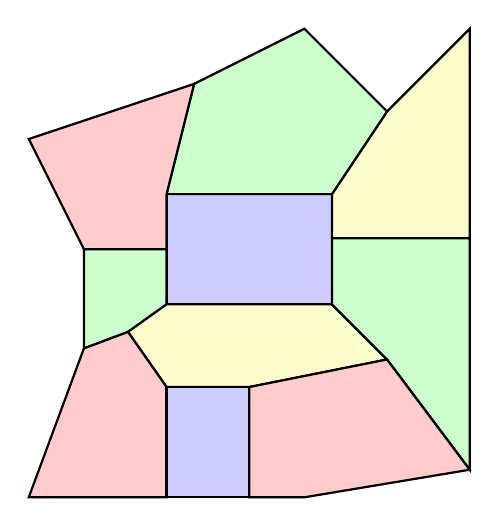
\begin{tikzpicture}[scale=0.7, thick, every node/.style={font=\tiny\bfseries}]
    % Map reproduction with shared coordinates
    \coordinate (P1) at (-1.5, 1);   % GL_NW
    \coordinate (P2) at (1.5, 1);    % GL_NE
    \coordinate (P3) at (1.5, -1);   % GL_SE
    \coordinate (P4) at (-1.5, -1);  % GL_SW
    \coordinate (C_GL_EAST_MID) at (1.5, 0.2); 
    \coordinate (C_GL_WEST_MID) at (-1.5, 0);  
    \coordinate (C_BK_HT) at (-1, 3);
    \coordinate (C_HT_EX) at (2.5, 2.5);
    \coordinate (C_EX_KT) at (4, 0.2);     
    \coordinate (C_KT_SR) at (2.5, -2);
    \coordinate (C_SR_ES) at (1, -2.3);
    \coordinate (C_ES_WS) at (0, -2.5);
    \coordinate (C_WS_HP) at (-1.5, -2.5);
    \coordinate (C_HP_BR) at (-3, -1.8);
    \coordinate (C_BR_BK) at (-3, 0);       
    \coordinate (C_BR_SR_HP) at (-2.2, -1.5); 
    \coordinate (C_HP_WS_B) at (-1.5, -4.5);  
    \coordinate (C_WS_ES_B) at (0, -4.5);     

    % 1. Greater London (GL) - Blue
    \draw[fill=blue!20] (P1) -- (P2) -- (C_GL_EAST_MID) -- (P3) -- (P4) -- (C_GL_WEST_MID) -- cycle;
    \node at (0,0) {};

    % 2. Essex (EX) - Yellow
    \draw[fill=yellow!20] (P2) -- (C_HT_EX) -- (4, 4) -- (C_EX_KT) -- (C_GL_EAST_MID) -- cycle;
    \node at (2.8, 1.8) {};

    % 3. Hertfordshire (HT) - Green
    \draw[fill=green!20] (P1) -- (C_BK_HT) -- (1, 4) -- (C_HT_EX) -- (P2) -- cycle;
    \node at (0.5, 2.5) {};

    % 4. Buckinghamshire (BK) - red
    \draw[fill=red!20] (P1) -- (C_GL_WEST_MID) -- (C_BR_BK) -- (-4, 2) -- (C_BK_HT) -- cycle;
    \node at (-2, 2.3) {};

    % 5. Berkshire (BR) - Green
    \draw[fill=green!20] (C_GL_WEST_MID) -- (P4) -- (C_BR_SR_HP) -- (C_HP_BR) -- (C_BR_BK) -- cycle;
    \node at (-2.5, -0.7) {};

    % 6. Surrey (SR) - Yellow
    \draw[fill=yellow!20] (P4) -- (P3) -- (C_KT_SR) -- (C_SR_ES) -- (C_ES_WS) -- (C_WS_HP) -- (C_BR_SR_HP) -- cycle;
    \node at (0.2, -1.8) {};

    % 7. Kent (KT) - Green
    \draw[fill=green!20] (P3) -- (C_GL_EAST_MID) -- (C_EX_KT) -- (4, -4) -- (C_KT_SR) -- cycle;
    \node at (3, -1) {};

    % 8. Hampshire (HP) - red
    \draw[fill=red!20] (C_BR_SR_HP) -- (C_WS_HP) -- (C_HP_WS_B) -- (-4, -4.5) -- (C_HP_BR) -- cycle;
    \node at (-2.8, -2.5) {};

    % 9. West Sussex (WS) - Blue
    \draw[fill=blue!20] (C_WS_HP) -- (C_ES_WS) -- (C_WS_ES_B) -- (C_HP_WS_B) -- cycle;
    \node at (-0.7, -3.5) {};

    % 10. East Sussex (ES) - red
    \draw[fill=red!20] (C_ES_WS) -- (C_SR_ES) -- (C_KT_SR) -- (4, -4) -- (1, -4.5) -- (C_WS_ES_B) -- cycle;
    \node at (1.8, -3.5) {};

\end{tikzpicture}
\hskip 2cm
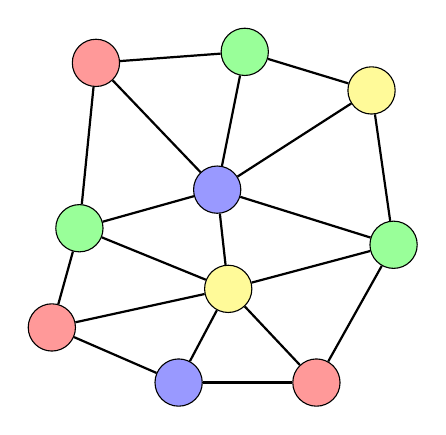
\begin{tikzpicture}[scale=0.7, every node/.style={circle, draw, minimum size=0.6cm, font=\tiny\bfseries}]
    % Dual Graph
    \node[fill=blue!40]   (V_GL) at (0,0){};
    \node[fill=yellow!40] (V_EX) at (2.8, 1.8) {};
    \node[fill=green!40]  (V_HT) at (0.5, 2.5) {};
    \node[fill=red!40] (V_BK) at (-2.2, 2.3) {};
    \node[fill=green!40]  (V_BR) at (-2.5, -0.7) {};
    \node[fill=yellow!40] (V_SR) at (0.2, -1.8) {};
    \node[fill=green!40]  (V_KT) at (3.2, -1) {};
    \node[fill=red!40] (V_HP) at (-3, -2.5) {};
    \node[fill=blue!40]   (V_WS) at (-0.7, -3.5) {};
    \node[fill=red!40] (V_ES) at (1.8, -3.5) {};
    
    % Adjacencies (Edges) - Solid Lines
    \draw[thick] (V_GL) -- (V_EX); \draw[thick] (V_GL) -- (V_HT); \draw[thick] (V_GL) -- (V_BK);
    \draw[thick] (V_GL) -- (V_BR); \draw[thick] (V_GL) -- (V_SR); \draw[thick] (V_GL) -- (V_KT);
    
    \draw[thick] (V_HT) -- (V_BK); \draw[thick] (V_HT) -- (V_EX);
    \draw[thick] (V_BK) -- (V_BR); \draw[thick] (V_EX) -- (V_KT);
    
    \draw[thick] (V_BR) -- (V_SR); \draw[thick] (V_BR) -- (V_HP);
    \draw[thick] (V_SR) -- (V_KT); \draw[thick] (V_SR) -- (V_ES); \draw[thick] (V_SR) -- (V_WS); \draw[thick] (V_SR) -- (V_HP);
    
    \draw[thick] (V_KT) -- (V_ES);
    \draw[thick] (V_HP) -- (V_WS); \draw[thick] (V_WS) -- (V_ES);
    
\end{tikzpicture}
\caption{A 4-coloured map and its 4-coloured dual graph}\label{dual}
\end{figure}

Rather than thinking about map colouring directly, we can look at the \emph{dual} problem (see Figure \ref{dual}). Each region in the map becomes a \emph{vertex} (a round node) and we draw an \emph{edge} (a straight line) between two vertices if their corresponding regions share a border. A colouring of the map is then equivalent to a colouring of the vertices of this dual graph, in which no two adjacent vertices have the same colour.

This dual object is called a \emph{planar graph}. The key property of a planar graph is that it can be drawn on a piece of paper without edge crossings (remember edges are the straight lines and vertices are the dots we colour).

Given any graph there are potentially many different ways to draw it. Some of these drawings may have edge crossings, but if the graph is planar then there will be at least one way to draw it without edge crossings.


If we look again at the example in Figure \ref{dual} it isn't hard to see that we can actually colour it with three colours, as shown in Figure \ref{3col}. 
\begin{figure}[h!]
\begin{center}
    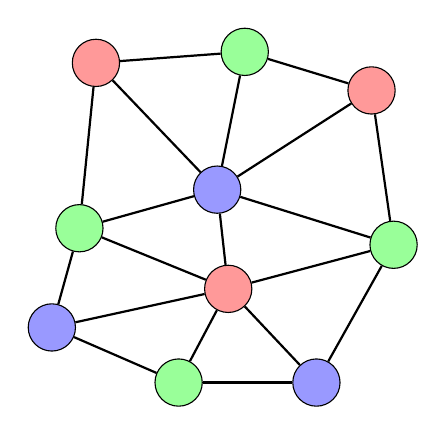
\begin{tikzpicture}[scale=0.7, every node/.style={circle, draw, minimum size=0.6cm, font=\tiny\bfseries}]
    % Dual Graph
    \node[fill=blue!40]   (V_GL) at (0,0) {};
    \node[fill=red!40] (V_EX) at (2.8, 1.8) {};
    \node[fill=green!40]  (V_HT) at (0.5, 2.5) {};
    \node[fill=red!40] (V_BK) at (-2.2, 2.3) {};
    \node[fill=green!40]  (V_BR) at (-2.5, -0.7) {};
    \node[fill=red!40] (V_SR) at (0.2, -1.8) {};
    \node[fill=green!40]  (V_KT) at (3.2, -1) {};
    \node[fill=blue!40] (V_HP) at (-3, -2.5) {};
    \node[fill=green!40]   (V_WS) at (-0.7, -3.5) {};
    \node[fill=blue!40] (V_ES) at (1.8, -3.5) {};
    
    % Adjacencies (Edges) - Solid Lines
    \draw[thick] (V_GL) -- (V_EX); \draw[thick] (V_GL) -- (V_HT); \draw[thick] (V_GL) -- (V_BK);
    \draw[thick] (V_GL) -- (V_BR); \draw[thick] (V_GL) -- (V_SR); \draw[thick] (V_GL) -- (V_KT);
    
    \draw[thick] (V_HT) -- (V_BK); \draw[thick] (V_HT) -- (V_EX);
    \draw[thick] (V_BK) -- (V_BR); \draw[thick] (V_EX) -- (V_KT);
    
    \draw[thick] (V_BR) -- (V_SR); \draw[thick] (V_BR) -- (V_HP);
    \draw[thick] (V_SR) -- (V_KT); \draw[thick] (V_SR) -- (V_ES); \draw[thick] (V_SR) -- (V_WS); \draw[thick] (V_SR) -- (V_HP);
    
    \draw[thick] (V_KT) -- (V_ES);
    \draw[thick] (V_HP) -- (V_WS); \draw[thick] (V_WS) -- (V_ES);
    
\end{tikzpicture}
\end{center}
\caption{A 3-colouring of the dual graph}\label{3col}
\end{figure}

The \emph{complete graph} on $t$ vertices, denoted $K_t$, is the graph in which every vertex is connected by an edge to every other vertex. For example $K_3$ is a triangle. If we want to colour the vertices of a complete graph so that no two adjacent vertices have the same colour, then we need to give each vertex a different colour. So $K_3$ needs 3 colours, $K_4$ needs 4 colours, and in general $K_t$ needs $t$ colours. 
\begin{question}
What is the largest complete graph $K_t$ that can be drawn in the plane without edge crossings?
\end{question}
(Note that this gives us a lower bound on the number of colours required to colour all planar graphs.)

\iffullversion
\textbf{Solution:\\}
We can certainly draw $K_4$ in the plane without any edges crossing, as shown in Figure \ref{K4}. However, if we try to draw $K_5$ we will find that no matter how we arrange the vertices and edges, at least one pair of edges will always cross. 
\begin{figure}[h]
\begin{center}
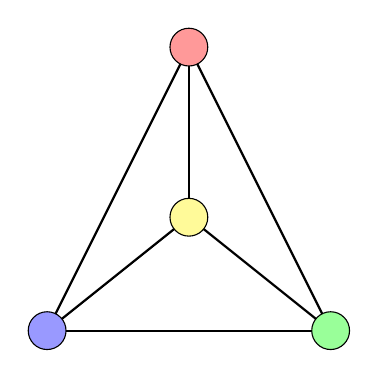
\begin{tikzpicture}[scale=1.2]
    % Define the four vertices - three forming a triangle, one in the center
    \coordinate (A) at (0,2);
    \coordinate (B) at (-1.5,-1);
    \coordinate (C) at (1.5,-1);
    \coordinate (D) at (0,0.2);
    
    % Draw all edges (complete graph K_4) - planar embedding
    \draw[thick] (A) -- (B);
    \draw[thick] (B) -- (C);
    \draw[thick] (C) -- (A);
    \draw[thick] (A) -- (D);
    \draw[thick] (B) -- (D);
    \draw[thick] (C) -- (D);
    
    % Draw vertices with 4 different colors
    \filldraw[fill=red!40, draw=black] (A) circle (0.2cm);
    \filldraw[fill=blue!40, draw=black] (B) circle (0.2cm);
    \filldraw[fill=green!40, draw=black] (C) circle (0.2cm);
    \filldraw[fill=yellow!40, draw=black] (D) circle (0.2cm);
\end{tikzpicture}
\end{center}
\caption{A 4-colouring of $K_4$ drawn in the plane}\label{K4}
\end{figure}
One way to see this is to first think about how $K_3$ can be drawn in the plane. It has 3 vertices, each pair are joined by an edge, so it is simply a triangle. If we want to add a fourth vertex, to create $K_4$, we can place it either inside or outside this triangle. However in both cases our drawing of $K_4$ will consist of a triangle with a single central vertex inside it, and the edges will subdivide the large triangle into three smaller triangles (so it looks something like Figure \ref{K4}).

How can we now add a fifth vertex? If we place it inside any of the smaller triangles then there is always one vertex that we cannot connect it to without edge crossings (namely the vertex not in the same triangle). If we place it outside the large triangle then we can't connect it to the central vertex without edge crossings. So we can't draw $K_5$ in the plane without edge crossings!


\fi

\section*{Doughnut Graphs}
\begin{figure}[!h]
\begin{center}
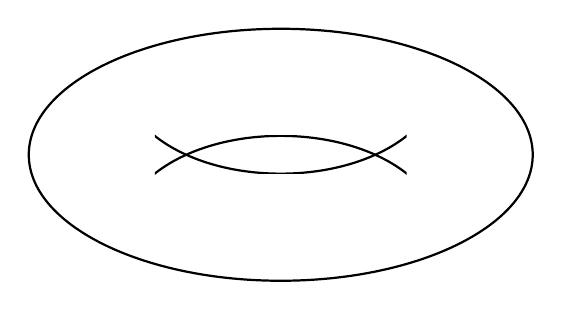
\begin{tikzpicture}[scale=0.8]
    % Torus schematic (isometric view)
    \draw[thick] (0,0) ellipse (4cm and 2cm);
    \begin{scope}
        \clip (-2,-0.3) rectangle (2,1);
        \draw[thick] (0,1.2) ellipse (2.5cm and 1.5cm);
    \end{scope}
    \begin{scope}
        \clip (-2,0.3) rectangle (2,-1);
        \draw[thick] (0,-1.2) ellipse (2.5cm and 1.5cm);
    \end{scope}
\end{tikzpicture}
\end{center}\caption{A doughnut (otherwise known as a torus)}\label{torus}
\end{figure}

% The question of how many colours are needed to colour a graph drawn on a doughnut (or \emph{torus} as mathematicians call it) is easier to answer than the planar case, but it still needs some rather fancy mathematics. 

% To start with let us try to find the largest complete graph $K_t$ that can be drawn properly on a torus (i.e.~with no edges crossings).

What if rather than drawing graphs in the plane we try to draw them on a doughnut or \emph{torus} as mathematicians call it? (See Figure \ref{torus}.) 

We can still ask the same question about colouring: how many colours do we need to colour the vertices of a graph drawn on a torus without edge crossings so that no two adjacent vertices have the same colour? We can get a lower bound on the number of colours required by answering the following question.
\begin{question}
What is the largest complete graph $K_t$ that can be drawn on a torus with no edge crossings?
\end{question}
Drawing a graph on a torus can be hard to visualize, but there is a nice trick we can use to help: we can draw the graph on a piece of paper and then roll it up into a cylinder, sticking the left and right edges together. We can can roll the cylinder up into a torus, sticking the top and bottom circles of the cylinder together. (In practice doing this by hand with a piece of paper is not easy, so here is an online tool to help you explore this problem \url{https://www.homepages.ucl.ac.uk/~ucahjmt/doughnut/} and find the answer.)


\iffullversion
\textbf{Solution:\\}
The largest complete graph that can be drawn properly on a torus is $K_7$. See Figures \ref{K7} and \ref{K7:3d} for 2D and 3D drawings.


\begin{figure}[h]
    \begin{center}
\input{tikz/2c.tikz}
            \end{center}
\caption{A drawing of $K_7$ on a torus (2D-version)}\label{K7}
        \end{figure}


\begin{figure}[h!]
    \begin{center}
% Requires: \usepackage{tikz,xcolor}
% Colors used: violet!60!blue for edges/vertices, orange!80!yellow for clique

% --- 3D Torus Projection ---
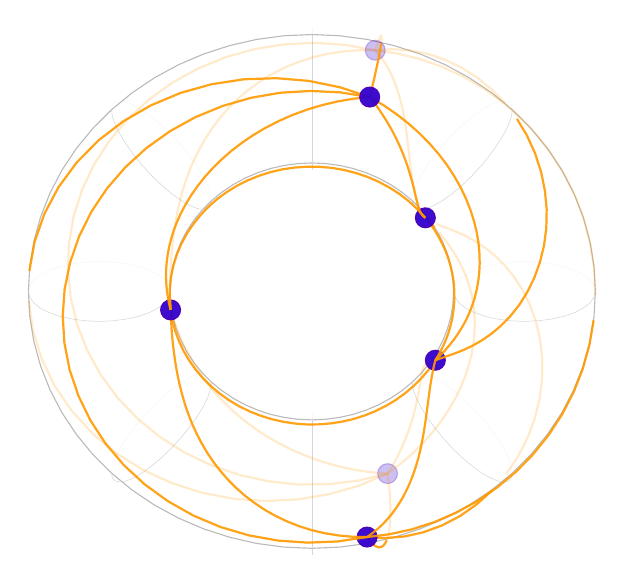
\begin{tikzpicture}[scale=0.9]
  \draw[gray!60, thin, opacity=0.9] (4.000,0.000) -- (3.981,0.355) -- (3.923,0.707) -- (3.828,1.052) -- (3.696,1.387) -- (3.528,1.709) -- (3.326,2.014) -- (3.092,2.300) -- (2.828,2.563) -- (2.538,2.802) -- (2.222,3.014) -- (1.886,3.197) -- (1.531,3.349) -- (1.161,3.469) -- (0.780,3.556) -- (0.392,3.608) -- (0.000,3.625) -- (-0.392,3.608) -- (-0.780,3.556) -- (-1.161,3.469) -- (-1.531,3.349) -- (-1.886,3.197) -- (-2.222,3.014) -- (-2.538,2.802) -- (-2.828,2.563) -- (-3.092,2.300) -- (-3.326,2.014) -- (-3.528,1.709) -- (-3.696,1.387) -- (-3.828,1.052) -- (-3.923,0.707) -- (-3.981,0.355) -- (-4.000,0.000) -- (-3.981,-0.355) -- (-3.923,-0.707) -- (-3.828,-1.052) -- (-3.696,-1.387) -- (-3.528,-1.709) -- (-3.326,-2.014) -- (-3.092,-2.300) -- (-2.828,-2.563) -- (-2.538,-2.802) -- (-2.222,-3.014) -- (-1.886,-3.197) -- (-1.531,-3.349) -- (-1.161,-3.469) -- (-0.780,-3.556) -- (-0.392,-3.608) -- (-0.000,-3.625) -- (0.392,-3.608) -- (0.780,-3.556) -- (1.161,-3.469) -- (1.531,-3.349) -- (1.886,-3.197) -- (2.222,-3.014) -- (2.538,-2.802) -- (2.828,-2.563) -- (3.092,-2.300) -- (3.326,-2.014) -- (3.528,-1.709) -- (3.696,-1.387) -- (3.828,-1.052) -- (3.923,-0.707) -- (3.981,-0.355) -- (4.000,-0.000);
  \draw[gray!60, thin, opacity=0.9] (2.000,-0.000) -- (1.990,0.178) -- (1.962,0.354) -- (1.914,0.526) -- (1.848,0.694) -- (1.764,0.854) -- (1.663,1.007) -- (1.546,1.150) -- (1.414,1.282) -- (1.269,1.401) -- (1.111,1.507) -- (0.943,1.599) -- (0.765,1.675) -- (0.581,1.735) -- (0.390,1.778) -- (0.196,1.804) -- (0.000,1.813) -- (-0.196,1.804) -- (-0.390,1.778) -- (-0.581,1.735) -- (-0.765,1.675) -- (-0.943,1.599) -- (-1.111,1.507) -- (-1.269,1.401) -- (-1.414,1.282) -- (-1.546,1.150) -- (-1.663,1.007) -- (-1.764,0.854) -- (-1.848,0.694) -- (-1.914,0.526) -- (-1.962,0.354) -- (-1.990,0.178) -- (-2.000,0.000) -- (-1.990,-0.178) -- (-1.962,-0.354) -- (-1.914,-0.526) -- (-1.848,-0.694) -- (-1.764,-0.854) -- (-1.663,-1.007) -- (-1.546,-1.150) -- (-1.414,-1.282) -- (-1.269,-1.401) -- (-1.111,-1.507) -- (-0.943,-1.599) -- (-0.765,-1.675) -- (-0.581,-1.735) -- (-0.390,-1.778) -- (-0.196,-1.804) -- (-0.000,-1.813) -- (0.196,-1.804) -- (0.390,-1.778) -- (0.581,-1.735) -- (0.765,-1.675) -- (0.943,-1.599) -- (1.111,-1.507) -- (1.269,-1.401) -- (1.414,-1.282) -- (1.546,-1.150) -- (1.663,-1.007) -- (1.764,-0.854) -- (1.848,-0.694) -- (1.914,-0.526) -- (1.962,-0.354) -- (1.990,-0.178) -- (2.000,-0.000);
  \draw[gray!35, very thin, opacity=0.9] (4.000,0.000) -- (3.981,-0.082) -- (3.924,-0.162) -- (3.831,-0.235) -- (3.707,-0.299) -- (3.556,-0.351) -- (3.383,-0.390) -- (3.195,-0.414) -- (3.000,-0.423) -- (2.805,-0.414) -- (2.617,-0.390) -- (2.444,-0.351) -- (2.293,-0.299) -- (2.169,-0.235) -- (2.076,-0.162) -- (2.019,-0.082) -- (2.000,-0.000);
  \draw[gray!35, very thin, opacity=0.2] (2.019,0.082) -- (2.076,0.162) -- (2.169,0.235) -- (2.293,0.299) -- (2.444,0.351) -- (2.617,0.390) -- (2.805,0.414) -- (3.000,0.423) -- (3.195,0.414) -- (3.383,0.390) -- (3.556,0.351) -- (3.707,0.299) -- (3.831,0.235) -- (3.924,0.162) -- (3.981,0.082) -- (4.000,0.000);
  \draw[gray!35, very thin, opacity=0.9] (2.828,2.563) -- (2.815,2.469) -- (2.775,2.353) -- (2.709,2.221) -- (2.621,2.077) -- (2.514,1.927) -- (2.392,1.777) -- (2.259,1.633) -- (2.121,1.500) -- (1.983,1.383) -- (1.851,1.287) -- (1.728,1.215) -- (1.621,1.171) -- (1.533,1.155) -- (1.468,1.169) -- (1.428,1.212) -- (1.414,1.282);
  \draw[gray!35, very thin, opacity=0.2] (1.428,1.376) -- (1.468,1.492) -- (1.533,1.625) -- (1.621,1.768) -- (1.728,1.918) -- (1.851,2.068) -- (1.983,2.212) -- (2.121,2.345) -- (2.259,2.462) -- (2.392,2.558) -- (2.514,2.630) -- (2.621,2.675) -- (2.709,2.690) -- (2.775,2.676) -- (2.815,2.634) -- (2.828,2.563);
  \draw[gray!35, very thin, opacity=0.9] (0.000,3.625) -- (0.000,3.525) -- (0.000,3.395) -- (0.000,3.238) -- (0.000,3.061) -- (0.000,2.871) -- (0.000,2.675) -- (0.000,2.481) -- (0.000,2.296) -- (0.000,2.128) -- (0.000,1.982) -- (0.000,1.864) -- (0.000,1.779) -- (0.000,1.731) -- (0.000,1.720) -- (0.000,1.748) -- (0.000,1.813);
  \draw[gray!35, very thin, opacity=0.2] (0.000,1.912) -- (0.000,2.043) -- (0.000,2.200) -- (0.000,2.377) -- (0.000,2.567) -- (0.000,2.763) -- (0.000,2.957) -- (0.000,3.142) -- (0.000,3.310) -- (0.000,3.456) -- (0.000,3.574) -- (0.000,3.659) -- (0.000,3.707) -- (0.000,3.718) -- (0.000,3.690) -- (0.000,3.625);
  \draw[gray!35, very thin, opacity=0.9] (-2.828,2.563) -- (-2.815,2.469) -- (-2.775,2.353) -- (-2.709,2.221) -- (-2.621,2.077) -- (-2.514,1.927) -- (-2.392,1.777) -- (-2.259,1.633) -- (-2.121,1.500) -- (-1.983,1.383) -- (-1.851,1.287) -- (-1.728,1.215) -- (-1.621,1.171) -- (-1.533,1.155) -- (-1.468,1.169) -- (-1.428,1.212) -- (-1.414,1.282);
  \draw[gray!35, very thin, opacity=0.2] (-1.428,1.376) -- (-1.468,1.492) -- (-1.533,1.625) -- (-1.621,1.768) -- (-1.728,1.918) -- (-1.851,2.068) -- (-1.983,2.212) -- (-2.121,2.345) -- (-2.259,2.462) -- (-2.392,2.558) -- (-2.514,2.630) -- (-2.621,2.675) -- (-2.709,2.690) -- (-2.775,2.676) -- (-2.815,2.634) -- (-2.828,2.563);
  \draw[gray!35, very thin, opacity=0.9] (-4.000,0.000) -- (-3.981,-0.082) -- (-3.924,-0.162) -- (-3.831,-0.235) -- (-3.707,-0.299) -- (-3.556,-0.351) -- (-3.383,-0.390) -- (-3.195,-0.414) -- (-3.000,-0.423) -- (-2.805,-0.414) -- (-2.617,-0.390) -- (-2.444,-0.351) -- (-2.293,-0.299) -- (-2.169,-0.235) -- (-2.076,-0.162) -- (-2.019,-0.082) -- (-2.000,0.000);
  \draw[gray!35, very thin, opacity=0.2] (-2.019,0.082) -- (-2.076,0.162) -- (-2.169,0.235) -- (-2.293,0.299) -- (-2.444,0.351) -- (-2.617,0.390) -- (-2.805,0.414) -- (-3.000,0.423) -- (-3.195,0.414) -- (-3.383,0.390) -- (-3.556,0.351) -- (-3.707,0.299) -- (-3.831,0.235) -- (-3.924,0.162) -- (-3.981,0.082) -- (-4.000,0.000);
  \draw[gray!35, very thin, opacity=0.9] (-2.828,-2.563) -- (-2.815,-2.634) -- (-2.775,-2.676) -- (-2.709,-2.690) -- (-2.621,-2.675) -- (-2.514,-2.630) -- (-2.392,-2.558) -- (-2.259,-2.462) -- (-2.121,-2.345) -- (-1.983,-2.212) -- (-1.851,-2.068) -- (-1.728,-1.918) -- (-1.621,-1.768) -- (-1.533,-1.625) -- (-1.468,-1.492) -- (-1.428,-1.376) -- (-1.414,-1.282);
  \draw[gray!35, very thin, opacity=0.2] (-1.428,-1.212) -- (-1.468,-1.169) -- (-1.533,-1.155) -- (-1.621,-1.171) -- (-1.728,-1.215) -- (-1.851,-1.287) -- (-1.983,-1.383) -- (-2.121,-1.500) -- (-2.259,-1.633) -- (-2.392,-1.777) -- (-2.514,-1.927) -- (-2.621,-2.077) -- (-2.709,-2.221) -- (-2.775,-2.353) -- (-2.815,-2.469) -- (-2.828,-2.563);
  \draw[gray!35, very thin, opacity=0.9] (-0.000,-3.625) -- (-0.000,-3.690) -- (-0.000,-3.718) -- (-0.000,-3.707) -- (-0.000,-3.659) -- (-0.000,-3.574) -- (-0.000,-3.456) -- (-0.000,-3.310) -- (-0.000,-3.142) -- (-0.000,-2.957) -- (-0.000,-2.763) -- (-0.000,-2.567) -- (-0.000,-2.377) -- (-0.000,-2.200) -- (-0.000,-2.043) -- (-0.000,-1.912) -- (-0.000,-1.813);
  \draw[gray!35, very thin, opacity=0.2] (-0.000,-1.748) -- (-0.000,-1.720) -- (-0.000,-1.731) -- (-0.000,-1.779) -- (-0.000,-1.864) -- (-0.000,-1.982) -- (-0.000,-2.128) -- (-0.000,-2.296) -- (-0.000,-2.481) -- (-0.000,-2.675) -- (-0.000,-2.871) -- (-0.000,-3.061) -- (-0.000,-3.238) -- (-0.000,-3.395) -- (-0.000,-3.525) -- (-0.000,-3.625);
  \draw[gray!35, very thin, opacity=0.9] (2.828,-2.563) -- (2.815,-2.634) -- (2.775,-2.676) -- (2.709,-2.690) -- (2.621,-2.675) -- (2.514,-2.630) -- (2.392,-2.558) -- (2.259,-2.462) -- (2.121,-2.345) -- (1.983,-2.212) -- (1.851,-2.068) -- (1.728,-1.918) -- (1.621,-1.768) -- (1.533,-1.625) -- (1.468,-1.492) -- (1.428,-1.376) -- (1.414,-1.282);
  \draw[gray!35, very thin, opacity=0.2] (1.428,-1.212) -- (1.468,-1.169) -- (1.533,-1.155) -- (1.621,-1.171) -- (1.728,-1.215) -- (1.851,-1.287) -- (1.983,-1.383) -- (2.121,-1.500) -- (2.259,-1.633) -- (2.392,-1.777) -- (2.514,-1.927) -- (2.621,-2.077) -- (2.709,-2.221) -- (2.775,-2.353) -- (2.815,-2.469) -- (2.828,-2.563);
  \filldraw[fill=violet!40!blue, draw=violet!60!blue, opacity=0.25] (1.068,-2.571) circle (4pt); % v6
  \draw[thick, orange!80!yellow, opacity=0.9] (0.779,-3.466) -- (0.803,-3.501) -- (0.827,-3.531) -- (0.851,-3.557) -- (0.874,-3.577) -- (0.896,-3.593) -- (0.918,-3.604) -- (0.939,-3.610) -- (0.959,-3.610) -- (0.978,-3.606) -- (0.996,-3.596) -- (1.013,-3.581) -- (1.029,-3.561) -- (1.043,-3.537) -- (1.056,-3.507);
  \draw[thick, orange!80!yellow, opacity=0.2] (1.068,-3.473) -- (1.078,-3.434) -- (1.087,-3.392) -- (1.095,-3.345) -- (1.100,-3.294) -- (1.105,-3.240) -- (1.108,-3.182) -- (1.109,-3.122) -- (1.109,-3.059) -- (1.107,-2.993) -- (1.104,-2.926) -- (1.100,-2.857) -- (1.094,-2.786) -- (1.087,-2.715) -- (1.078,-2.643) -- (1.068,-2.571);
  \draw[thick, orange!80!yellow, opacity=0.2] (1.068,-2.571) -- (1.125,-2.478) -- (1.178,-2.385) -- (1.226,-2.292) -- (1.270,-2.199) -- (1.310,-2.108) -- (1.345,-2.019) -- (1.377,-1.932) -- (1.405,-1.847) -- (1.429,-1.765) -- (1.450,-1.687) -- (1.468,-1.612) -- (1.483,-1.541) -- (1.496,-1.474) -- (1.508,-1.411) -- (1.517,-1.352) -- (1.526,-1.298) -- (1.533,-1.249) -- (1.541,-1.204) -- (1.548,-1.164) -- (1.556,-1.129) -- (1.565,-1.097) -- (1.575,-1.070) -- (1.587,-1.047) -- (1.601,-1.028) -- (1.617,-1.012) -- (1.636,-0.999) -- (1.657,-0.989);
  \draw[thick, orange!80!yellow, opacity=0.9] (1.682,-0.981) -- (1.710,-0.975) -- (1.742,-0.971);
  \draw[thick, orange!80!yellow, opacity=0.9] (-1.994,-0.261) -- (-1.971,-0.336);
  \draw[thick, orange!80!yellow, opacity=0.2] (-1.946,-0.411) -- (-1.919,-0.485) -- (-1.890,-0.560) -- (-1.859,-0.635) -- (-1.825,-0.712) -- (-1.787,-0.791) -- (-1.746,-0.872) -- (-1.701,-0.955) -- (-1.650,-1.040) -- (-1.594,-1.128) -- (-1.532,-1.218) -- (-1.463,-1.311) -- (-1.387,-1.405) -- (-1.302,-1.500) -- (-1.208,-1.597) -- (-1.106,-1.694) -- (-0.994,-1.790) -- (-0.872,-1.885) -- (-0.740,-1.978) -- (-0.598,-2.068) -- (-0.446,-2.153) -- (-0.284,-2.234) -- (-0.113,-2.308) -- (0.066,-2.376) -- (0.254,-2.435) -- (0.449,-2.485) -- (0.651,-2.525) -- (0.858,-2.554) -- (1.068,-2.571);
  \draw[thick, orange!80!yellow, opacity=0.9] (1.601,1.039) -- (1.668,0.971) -- (1.732,0.902);
  \draw[thick, orange!80!yellow, opacity=0.2] (1.794,0.832) -- (1.853,0.760) -- (1.910,0.685) -- (1.965,0.608) -- (2.017,0.528) -- (2.067,0.443) -- (2.114,0.353) -- (2.157,0.258) -- (2.196,0.157) -- (2.229,0.050) -- (2.258,-0.063) -- (2.279,-0.182) -- (2.293,-0.308) -- (2.299,-0.441) -- (2.295,-0.579) -- (2.281,-0.723) -- (2.256,-0.873) -- (2.218,-1.026) -- (2.168,-1.184) -- (2.104,-1.344) -- (2.026,-1.505) -- (1.933,-1.667) -- (1.826,-1.828) -- (1.704,-1.987) -- (1.566,-2.142) -- (1.414,-2.292) -- (1.248,-2.435) -- (1.068,-2.571);
  \draw[thick, orange!80!yellow, opacity=0.2] (1.068,-2.571) -- (0.657,-2.669) -- (0.236,-2.720) -- (-0.189,-2.724) -- (-0.611,-2.680) -- (-1.025,-2.589) -- (-1.423,-2.452) -- (-1.799,-2.272) -- (-2.148,-2.051) -- (-2.464,-1.792) -- (-2.742,-1.500) -- (-2.978,-1.179) -- (-3.169,-0.834) -- (-3.311,-0.469) -- (-3.402,-0.092) -- (-3.442,0.293) -- (-3.428,0.679) -- (-3.362,1.061) -- (-3.243,1.433) -- (-3.076,1.788) -- (-2.860,2.123) -- (-2.601,2.430) -- (-2.301,2.706) -- (-1.967,2.947) -- (-1.601,3.148) -- (-1.211,3.307) -- (-0.802,3.421) -- (-0.381,3.488) -- (0.047,3.508) -- (0.474,3.479) -- (0.894,3.403);
  \draw[thick, orange!80!yellow, opacity=0.9] (1.601,1.039) -- (1.669,0.995);
  \draw[thick, orange!80!yellow, opacity=0.2] (1.746,0.957) -- (1.835,0.921) -- (1.936,0.882) -- (2.049,0.837) -- (2.172,0.781) -- (2.305,0.708) -- (2.443,0.617) -- (2.583,0.505) -- (2.722,0.368) -- (2.853,0.206) -- (2.974,0.019) -- (3.078,-0.192) -- (3.162,-0.425) -- (3.220,-0.678) -- (3.250,-0.945) -- (3.249,-1.223) -- (3.215,-1.507) -- (3.146,-1.791) -- (3.043,-2.068) -- (2.907,-2.333) -- (2.740,-2.581);
  \draw[thick, orange!80!yellow, opacity=0.9] (2.545,-2.806) -- (2.326,-3.004) -- (2.088,-3.171) -- (1.834,-3.303) -- (1.572,-3.399) -- (1.305,-3.458) -- (1.039,-3.480) -- (0.779,-3.466);
  \filldraw[fill=violet!40!blue, draw=violet!60!blue, opacity=0.95] (0.779,-3.466) circle (4pt); % v2
  \draw[thick, orange!80!yellow, opacity=0.9] (-1.994,-0.261) -- (-1.968,-0.411) -- (-1.928,-0.559) -- (-1.875,-0.703) -- (-1.809,-0.843) -- (-1.730,-0.977) -- (-1.639,-1.105) -- (-1.537,-1.225) -- (-1.424,-1.338) -- (-1.301,-1.441) -- (-1.169,-1.535) -- (-1.029,-1.619) -- (-0.882,-1.691) -- (-0.728,-1.752) -- (-0.569,-1.802) -- (-0.407,-1.839) -- (-0.242,-1.864) -- (-0.074,-1.877) -- (0.093,-1.876) -- (0.260,-1.863) -- (0.425,-1.838) -- (0.588,-1.800) -- (0.746,-1.750) -- (0.899,-1.688) -- (1.045,-1.615) -- (1.185,-1.531) -- (1.316,-1.436) -- (1.438,-1.332) -- (1.550,-1.220) -- (1.652,-1.099) -- (1.742,-0.971);
  \filldraw[fill=violet!40!blue, draw=violet!60!blue, opacity=0.95] (1.742,-0.971) circle (4pt); % v4
  \draw[thick, orange!80!yellow, opacity=0.9] (1.742,-0.971) -- (1.723,-1.046) -- (1.707,-1.124) -- (1.692,-1.202) -- (1.678,-1.283) -- (1.666,-1.364) -- (1.654,-1.448) -- (1.643,-1.533) -- (1.631,-1.619) -- (1.620,-1.707) -- (1.608,-1.796) -- (1.595,-1.886) -- (1.580,-1.978) -- (1.564,-2.070) -- (1.546,-2.162) -- (1.526,-2.255) -- (1.503,-2.348) -- (1.476,-2.441) -- (1.447,-2.533) -- (1.414,-2.624) -- (1.378,-2.714) -- (1.337,-2.802) -- (1.293,-2.889) -- (1.244,-2.973) -- (1.191,-3.054) -- (1.133,-3.133) -- (1.071,-3.208) -- (1.005,-3.279) -- (0.934,-3.346) -- (0.858,-3.408) -- (0.779,-3.466);
  \draw[thick, orange!80!yellow, opacity=0.9] (-1.994,-0.261) -- (-1.988,-0.391) -- (-1.980,-0.521) -- (-1.970,-0.653) -- (-1.956,-0.785) -- (-1.939,-0.918) -- (-1.919,-1.052) -- (-1.894,-1.187) -- (-1.865,-1.323) -- (-1.830,-1.459) -- (-1.790,-1.596) -- (-1.743,-1.733) -- (-1.689,-1.870) -- (-1.627,-2.006) -- (-1.557,-2.140) -- (-1.479,-2.273) -- (-1.392,-2.403) -- (-1.295,-2.529) -- (-1.189,-2.651) -- (-1.074,-2.768) -- (-0.948,-2.879) -- (-0.813,-2.983) -- (-0.668,-3.080) -- (-0.514,-3.167) -- (-0.351,-3.245) -- (-0.180,-3.313) -- (-0.001,-3.369) -- (0.186,-3.413) -- (0.378,-3.444) -- (0.577,-3.462) -- (0.779,-3.466);
  \draw[thick, orange!80!yellow, opacity=0.9] (0.816,2.743) -- (0.396,2.881) -- (-0.045,2.971) -- (-0.498,3.009) -- (-0.956,2.994) -- (-1.410,2.925) -- (-1.851,2.802) -- (-2.271,2.626) -- (-2.661,2.401) -- (-3.013,2.130) -- (-3.320,1.818) -- (-3.576,1.470) -- (-3.775,1.095) -- (-3.913,0.698) -- (-3.987,0.287);
  \draw[thick, orange!80!yellow, opacity=0.2] (-3.995,-0.128) -- (-3.938,-0.541) -- (-3.817,-0.941) -- (-3.635,-1.323) -- (-3.394,-1.678) -- (-3.102,-1.999) -- (-2.762,-2.281) -- (-2.384,-2.518) -- (-1.974,-2.706) -- (-1.541,-2.843) -- (-1.093,-2.927) -- (-0.640,-2.957) -- (-0.189,-2.934) -- (0.251,-2.860) -- (0.673,-2.738) -- (1.068,-2.571);
  \draw[thick, orange!80!yellow, opacity=0.2] (0.894,3.403) -- (1.207,3.357) -- (1.520,3.281) -- (1.829,3.173) -- (2.130,3.035) -- (2.420,2.867) -- (2.696,2.669) -- (2.952,2.444) -- (3.187,2.193) -- (3.397,1.918) -- (3.579,1.622) -- (3.731,1.309) -- (3.850,0.981) -- (3.935,0.641) -- (3.985,0.295) -- (3.999,-0.056);
  \draw[thick, orange!80!yellow, opacity=0.9] (3.976,-0.406) -- (3.917,-0.752) -- (3.823,-1.090) -- (3.695,-1.417) -- (3.535,-1.728) -- (3.344,-2.022) -- (3.126,-2.294) -- (2.883,-2.542) -- (2.618,-2.763) -- (2.335,-2.957) -- (2.038,-3.121) -- (1.730,-3.254) -- (1.415,-3.356) -- (1.097,-3.426) -- (0.779,-3.466);
  \filldraw[fill=violet!40!blue, draw=violet!60!blue, opacity=0.95] (-1.994,-0.261) circle (4pt); % v7
  \draw[thick, orange!80!yellow, opacity=0.9] (-1.994,-0.261) -- (-1.999,-0.112);
  \draw[thick, orange!80!yellow, opacity=0.2] (-2.000,0.036) -- (-1.998,0.184) -- (-1.993,0.333) -- (-1.984,0.482) -- (-1.971,0.632) -- (-1.954,0.783) -- (-1.932,0.935) -- (-1.905,1.088) -- (-1.872,1.242) -- (-1.831,1.396) -- (-1.783,1.551) -- (-1.727,1.706) -- (-1.662,1.860) -- (-1.586,2.012) -- (-1.500,2.162) -- (-1.403,2.309) -- (-1.295,2.452) -- (-1.174,2.590) -- (-1.041,2.721) -- (-0.896,2.844) -- (-0.738,2.959) -- (-0.569,3.063) -- (-0.388,3.156) -- (-0.196,3.236) -- (0.006,3.302) -- (0.218,3.352) -- (0.437,3.386) -- (0.663,3.404) -- (0.894,3.403);
  \draw[thick, orange!80!yellow, opacity=0.9] (1.742,-0.971) -- (1.780,-0.909) -- (1.815,-0.845) -- (1.847,-0.780) -- (1.877,-0.714) -- (1.904,-0.648) -- (1.928,-0.580) -- (1.949,-0.511) -- (1.967,-0.442) -- (1.982,-0.372) -- (1.993,-0.302) -- (2.002,-0.231) -- (2.008,-0.160) -- (2.011,-0.089) -- (2.010,-0.018) -- (2.007,0.053) -- (2.001,0.124) -- (1.991,0.195) -- (1.978,0.265) -- (1.963,0.334) -- (1.944,0.404) -- (1.923,0.472) -- (1.898,0.540) -- (1.871,0.606) -- (1.840,0.672) -- (1.807,0.736) -- (1.771,0.800) -- (1.733,0.862) -- (1.691,0.922) -- (1.648,0.981) -- (1.601,1.039);
  \draw[thick, orange!80!yellow, opacity=0.2] (0.894,3.403) -- (0.949,3.339) -- (0.999,3.272) -- (1.046,3.200) -- (1.089,3.124) -- (1.128,3.045) -- (1.163,2.963) -- (1.195,2.878) -- (1.223,2.791) -- (1.248,2.703) -- (1.270,2.613) -- (1.290,2.523) -- (1.306,2.432) -- (1.321,2.341) -- (1.334,2.250) -- (1.345,2.160) -- (1.356,2.071) -- (1.366,1.983) -- (1.375,1.896) -- (1.385,1.812) -- (1.395,1.729) -- (1.406,1.649) -- (1.418,1.571) -- (1.432,1.495) -- (1.448,1.422) -- (1.466,1.352) -- (1.486,1.284) -- (1.510,1.219);
  \draw[thick, orange!80!yellow, opacity=0.9] (1.537,1.156) -- (1.567,1.096) -- (1.601,1.039);
  \filldraw[fill=violet!40!blue, draw=violet!60!blue, opacity=0.25] (0.894,3.403) circle (4pt); % v5
  \filldraw[fill=violet!40!blue, draw=violet!60!blue, opacity=0.95] (1.601,1.039) circle (4pt); % v3
  \draw[thick, orange!80!yellow, opacity=0.9] (-1.994,-0.261) -- (-2.007,-0.104) -- (-2.004,0.054) -- (-1.987,0.211) -- (-1.954,0.366) -- (-1.907,0.517) -- (-1.845,0.665) -- (-1.769,0.807) -- (-1.680,0.942) -- (-1.578,1.070) -- (-1.465,1.190) -- (-1.340,1.300) -- (-1.205,1.400) -- (-1.061,1.489) -- (-0.909,1.566) -- (-0.750,1.631) -- (-0.586,1.683) -- (-0.417,1.723) -- (-0.245,1.748) -- (-0.071,1.760) -- (0.104,1.759) -- (0.278,1.744) -- (0.449,1.715) -- (0.618,1.672) -- (0.782,1.617) -- (0.940,1.549) -- (1.090,1.468) -- (1.233,1.377) -- (1.366,1.274) -- (1.489,1.161) -- (1.601,1.039);
  \draw[thick, orange!80!yellow, opacity=0.9] (0.816,2.743) -- (0.400,2.809) -- (-0.021,2.829) -- (-0.443,2.804) -- (-0.857,2.733) -- (-1.259,2.617) -- (-1.644,2.459) -- (-2.004,2.260) -- (-2.335,2.023) -- (-2.633,1.752) -- (-2.893,1.451) -- (-3.112,1.124) -- (-3.285,0.776) -- (-3.411,0.411) -- (-3.489,0.035) -- (-3.516,-0.346) -- (-3.492,-0.728) -- (-3.419,-1.104) -- (-3.296,-1.469) -- (-3.126,-1.819) -- (-2.911,-2.147) -- (-2.654,-2.450) -- (-2.359,-2.723) -- (-2.030,-2.961) -- (-1.672,-3.163) -- (-1.290,-3.324) -- (-0.890,-3.442) -- (-0.477,-3.516) -- (-0.057,-3.545) -- (0.364,-3.528) -- (0.779,-3.466);
  \draw[thick, orange!80!yellow, opacity=0.2] (0.894,3.403) -- (1.133,3.418) -- (1.378,3.402) -- (1.624,3.355) -- (1.867,3.275) -- (2.103,3.163) -- (2.328,3.021) -- (2.537,2.850) -- (2.727,2.654);
  \draw[thick, orange!80!yellow, opacity=0.9] (2.894,2.435) -- (3.036,2.198) -- (3.150,1.947) -- (3.234,1.687) -- (3.288,1.423) -- (3.313,1.158) -- (3.308,0.899) -- (3.276,0.649) -- (3.218,0.413) -- (3.139,0.193) -- (3.040,-0.008) -- (2.927,-0.189) -- (2.802,-0.347) -- (2.670,-0.482) -- (2.534,-0.597) -- (2.399,-0.690) -- (2.268,-0.765) -- (2.143,-0.825) -- (2.026,-0.871) -- (1.920,-0.909) -- (1.825,-0.941) -- (1.742,-0.971);
  \draw[thick, orange!80!yellow, opacity=0.9] (1.742,-0.971) -- (1.811,-0.903) -- (1.878,-0.833) -- (1.942,-0.758) -- (2.004,-0.680) -- (2.062,-0.597) -- (2.117,-0.509) -- (2.169,-0.416) -- (2.216,-0.317) -- (2.258,-0.212) -- (2.294,-0.102) -- (2.324,0.015) -- (2.347,0.138) -- (2.362,0.267) -- (2.368,0.401) -- (2.364,0.541) -- (2.351,0.686) -- (2.326,0.835) -- (2.289,0.988) -- (2.240,1.143) -- (2.178,1.301) -- (2.103,1.460) -- (2.014,1.618) -- (1.912,1.776) -- (1.795,1.931) -- (1.665,2.082) -- (1.520,2.229) -- (1.363,2.370) -- (1.192,2.503) -- (1.010,2.628) -- (0.816,2.743);
  \draw[thick, orange!80!yellow, opacity=0.9] (-1.994,-0.261) -- (-2.015,-0.173) -- (-2.032,-0.083) -- (-2.046,0.009) -- (-2.054,0.104) -- (-2.058,0.202) -- (-2.057,0.303) -- (-2.049,0.408) -- (-2.035,0.516) -- (-2.015,0.627) -- (-1.986,0.743) -- (-1.949,0.861) -- (-1.903,0.982) -- (-1.847,1.106) -- (-1.780,1.231) -- (-1.703,1.358) -- (-1.614,1.485) -- (-1.514,1.612) -- (-1.401,1.738) -- (-1.276,1.861) -- (-1.139,1.981) -- (-0.989,2.096) -- (-0.828,2.206) -- (-0.655,2.308) -- (-0.471,2.403) -- (-0.276,2.489) -- (-0.072,2.564) -- (0.140,2.628) -- (0.360,2.680) -- (0.585,2.719) -- (0.816,2.743);
  \draw[thick, orange!80!yellow, opacity=0.9] (0.816,2.743) -- (0.833,2.811) -- (0.849,2.878) -- (0.865,2.943) -- (0.880,3.008) -- (0.894,3.070) -- (0.907,3.130) -- (0.920,3.188) -- (0.931,3.243) -- (0.942,3.295) -- (0.951,3.343) -- (0.959,3.388) -- (0.966,3.430) -- (0.972,3.467) -- (0.977,3.500);
  \draw[thick, orange!80!yellow, opacity=0.2] (0.981,3.529) -- (0.983,3.554) -- (0.984,3.574) -- (0.984,3.589) -- (0.983,3.599) -- (0.980,3.605) -- (0.976,3.606) -- (0.971,3.602) -- (0.965,3.593) -- (0.958,3.579) -- (0.950,3.561) -- (0.940,3.538) -- (0.930,3.511) -- (0.919,3.479) -- (0.907,3.443) -- (0.894,3.403);
  \draw[thick, orange!80!yellow, opacity=0.9] (0.816,2.743) -- (0.880,2.662) -- (0.940,2.580) -- (0.996,2.496) -- (1.049,2.413) -- (1.098,2.330) -- (1.144,2.247) -- (1.186,2.164) -- (1.225,2.083) -- (1.260,2.004) -- (1.292,1.926) -- (1.320,1.851) -- (1.346,1.778) -- (1.369,1.707) -- (1.389,1.640) -- (1.407,1.576) -- (1.424,1.515) -- (1.438,1.457) -- (1.451,1.403) -- (1.462,1.353) -- (1.473,1.307) -- (1.484,1.264) -- (1.494,1.225) -- (1.504,1.190) -- (1.514,1.159) -- (1.525,1.131) -- (1.537,1.106) -- (1.551,1.085) -- (1.566,1.067) -- (1.583,1.052) -- (1.601,1.039);
  \filldraw[fill=violet!40!blue, draw=violet!60!blue, opacity=0.95] (0.816,2.743) circle (4pt); % v1
\end{tikzpicture}
            \end{center}
\caption{A drawing of $K_7$ on a torus (3D-version)}\label{K7:3d}
        \end{figure}

To see why $K_8$ cannot be drawn on a torus without edges crossing, we need to use a magical formula (called the \emph{Euler characteristic}) that tells us how the number of vertices ($V$), edges ($E$), and faces ($F$) of a graph drawn on a surface are related. This formula is an invariant of the surface (which means that it is true for all graphs drawn on the same surface). For a torus the formula says that: 
\begin{equation}\label{EC:eq}
V- E+ F \ge 0.
\end{equation}

We also need to use the fact that if a graph has at least 3 edges and is \emph{connected} (this just means we can travel between any two vertices by following edges) then $F \le 2E/3$. (This is essentially because every face of such a graph contains at least 3 edges, and each edge belongs to at most 2 faces.)

Putting these two facts together we can check whether $K_8$ can be drawn on a torus without edge crossings. Since $K_8$ has 8 vertices and $\binom{8}{2} = 28$ edges, if we could draw it on a torus without edge crossings then, using the inequality $F \le 2E/3$, we have 
\[F \le \frac{2E}{3} = \frac{2 \cdot 28}{3} = \frac{56}{3}.\] But then  \[V - E + F \le 8 - 28 + \frac{56}{3} = -\frac{4}{3} < 0,\] which contradicts the Euler characteristic bound (\ref{EC:eq}). So $K_8$ cannot be drawn on a torus without edges crossing.

[This argument can actually be adapted to prove the \emph{Seven Colour Theorem}, which says that any graph drawn without edge crossings on a torus can be coloured using 7 colours. The basic idea is that you can show that any graph drawn on a torus has at least one vertex that has at most 6 neighbours. You can remove that vertex and colour the rest of the graph using 7 colours (by induction!), and then add the vertex back in and colour it using one of the 7 colours that is not used by any of its neighbours.]
\fi

\subsection*{Utility Graphs}
The \emph{utility} graph $K_{t,t}$ is the graph that consists of two sets of $t$ vertices with edges between any pair of vertices from different classes. (See Figure \ref{utility_graphs}.)
\begin{figure}[h!]
\begin{center}
    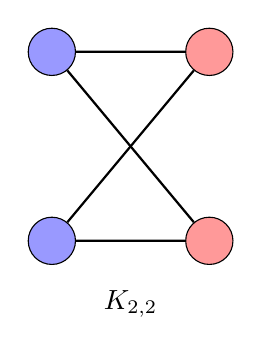
\begin{tikzpicture}[scale=0.8, every node/.style={circle, draw, minimum size=0.6cm}]
        % K_{2,2}
        \node[fill=blue!40] (A1) at (0, 1.5) {};
        \node[fill=blue!40] (A2) at (0, -1.5) {};
        \node[fill=red!40] (B1) at (2.5, 1.5) {};
        \node[fill=red!40] (B2) at (2.5, -1.5) {};
        
        \draw[thick] (A1) -- (B1);
        \draw[thick] (A1) -- (B2);
        \draw[thick] (A2) -- (B1);
        \draw[thick] (A2) -- (B2);
        
        \node[draw=none, fill=none, rectangle] at (1.25, -2.5) {$K_{2,2}$};
    \end{tikzpicture}
    \hskip 3cm
    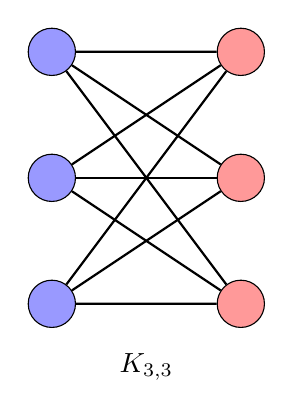
\begin{tikzpicture}[scale=0.8, every node/.style={circle, draw, minimum size=0.6cm}]
        % K_{3,3}
        \node[fill=blue!40] (A1) at (0, 2) {};
        \node[fill=blue!40] (A2) at (0, 0) {};
        \node[fill=blue!40] (A3) at (0, -2) {};
        
        \node[fill=red!40] (B1) at (3, 2) {};
        \node[fill=red!40] (B2) at (3, 0) {};
        \node[fill=red!40] (B3) at (3, -2) {};
        
        \draw[thick] (A1) -- (B1); \draw[thick] (A1) -- (B2); \draw[thick] (A1) -- (B3);
        \draw[thick] (A2) -- (B1); \draw[thick] (A2) -- (B2); \draw[thick] (A2) -- (B3);
        \draw[thick] (A3) -- (B1); \draw[thick] (A3) -- (B2); \draw[thick] (A3) -- (B3);
        
        \node[draw=none, fill=none, rectangle] at (1.5, -3) {$K_{3,3}$};
    \end{tikzpicture}
\end{center}
\caption{The utility graphs $K_{2,2}$ and $K_{3,3}$}\label{utility_graphs}
\end{figure}
% You should be able to easily convince yourself that $K_{2,2}$ can be drawn without edge crossings in the plane. (You could also try to convince yourself that $K_{3,3}$ cannot be drawn without edge crossings in the plane.)
\begin{question}
What is the largest utility graph you can draw on the torus without edge crossings?
\end{question}
\iffullversion
\textbf{Solution:\\}
We can draw $K_{4,4}$ on the torus with edge crossings (see Figures \ref{K44} and \ref{K44:3d}) but not $K_{5,5}$. 
\begin{figure}[h]
    \begin{center}
% Requires: \usepackage{tikz,xcolor}
% Colors used: violet!60!blue for edges/vertices, orange!80!yellow for clique

% --- 2D Flat Torus Representation ---
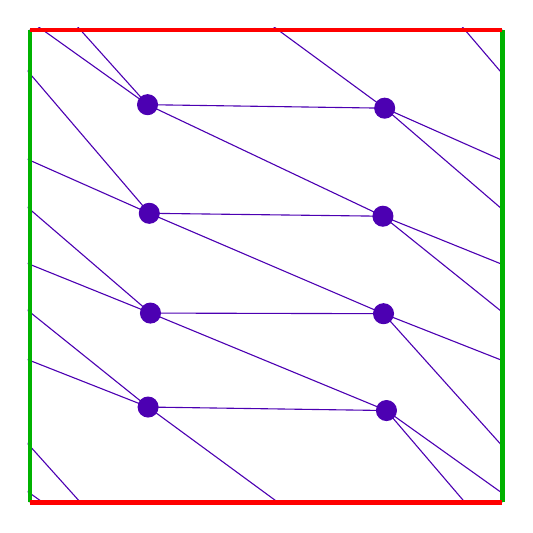
\begin{tikzpicture}[scale=6]
  \draw[gray!40, thin] (0,0) rectangle (1,1);
  \begin{scope}
    \clip (-0.005,-0.005) rectangle (1.005,1.005);
    \draw[violet!60!blue] (-0.7513,1.8420) -- (-0.2493,1.8346);
    \draw[violet!60!blue] (-0.7513,0.8420) -- (-0.2493,0.8346);
    \draw[violet!60!blue] (-0.7513,-0.1580) -- (-0.2493,-0.1654);
    \draw[violet!60!blue] (0.2487,1.8420) -- (0.7507,1.8346);
    \draw[violet!60!blue] (0.2487,0.8420) -- (0.7507,0.8346);
    \draw[violet!60!blue] (0.2487,-0.1580) -- (0.7507,-0.1654);
    \draw[violet!60!blue] (1.2487,1.8420) -- (1.7507,1.8346);
    \draw[violet!60!blue] (1.2487,0.8420) -- (1.7507,0.8346);
    \draw[violet!60!blue] (1.2487,-0.1580) -- (1.7507,-0.1654);
    \draw[violet!60!blue] (-0.7513,1.8420) -- (-0.2530,1.6059);
    \draw[violet!60!blue] (-0.7513,0.8420) -- (-0.2530,0.6059);
    \draw[violet!60!blue] (-0.7513,-0.1580) -- (-0.2530,-0.3941);
    \draw[violet!60!blue] (0.2487,1.8420) -- (0.7470,1.6059);
    \draw[violet!60!blue] (0.2487,0.8420) -- (0.7470,0.6059);
    \draw[violet!60!blue] (0.2487,-0.1580) -- (0.7470,-0.3941);
    \draw[violet!60!blue] (1.2487,1.8420) -- (1.7470,1.6059);
    \draw[violet!60!blue] (1.2487,0.8420) -- (1.7470,0.6059);
    \draw[violet!60!blue] (1.2487,-0.1580) -- (1.7470,-0.3941);
    \draw[violet!60!blue] (-0.7476,1.6121) -- (-0.2530,1.6059);
    \draw[violet!60!blue] (-0.7476,0.6121) -- (-0.2530,0.6059);
    \draw[violet!60!blue] (-0.7476,-0.3879) -- (-0.2530,-0.3941);
    \draw[violet!60!blue] (0.2524,1.6121) -- (0.7470,1.6059);
    \draw[violet!60!blue] (0.2524,0.6121) -- (0.7470,0.6059);
    \draw[violet!60!blue] (0.2524,-0.3879) -- (0.7470,-0.3941);
    \draw[violet!60!blue] (1.2524,1.6121) -- (1.7470,1.6059);
    \draw[violet!60!blue] (1.2524,0.6121) -- (1.7470,0.6059);
    \draw[violet!60!blue] (1.2524,-0.3879) -- (1.7470,-0.3941);
    \draw[violet!60!blue] (-0.7476,1.6121) -- (-0.2518,1.3996);
    \draw[violet!60!blue] (-0.7476,0.6121) -- (-0.2518,0.3996);
    \draw[violet!60!blue] (-0.7476,-0.3879) -- (-0.2518,-0.6004);
    \draw[violet!60!blue] (0.2524,1.6121) -- (0.7482,1.3996);
    \draw[violet!60!blue] (0.2524,0.6121) -- (0.7482,0.3996);
    \draw[violet!60!blue] (0.2524,-0.3879) -- (0.7482,-0.6004);
    \draw[violet!60!blue] (1.2524,1.6121) -- (1.7482,1.3996);
    \draw[violet!60!blue] (1.2524,0.6121) -- (1.7482,0.3996);
    \draw[violet!60!blue] (1.2524,-0.3879) -- (1.7482,-0.6004);
    \draw[violet!60!blue] (-0.7451,1.4009) -- (-0.2518,1.3996);
    \draw[violet!60!blue] (-0.7451,0.4009) -- (-0.2518,0.3996);
    \draw[violet!60!blue] (-0.7451,-0.5991) -- (-0.2518,-0.6004);
    \draw[violet!60!blue] (0.2549,1.4009) -- (0.7482,1.3996);
    \draw[violet!60!blue] (0.2549,0.4009) -- (0.7482,0.3996);
    \draw[violet!60!blue] (0.2549,-0.5991) -- (0.7482,-0.6004);
    \draw[violet!60!blue] (1.2549,1.4009) -- (1.7482,1.3996);
    \draw[violet!60!blue] (1.2549,0.4009) -- (1.7482,0.3996);
    \draw[violet!60!blue] (1.2549,-0.5991) -- (1.7482,-0.6004);
    \draw[violet!60!blue] (-0.7451,1.4009) -- (-0.2456,1.1946);
    \draw[violet!60!blue] (-0.7451,0.4009) -- (-0.2456,0.1946);
    \draw[violet!60!blue] (-0.7451,-0.5991) -- (-0.2456,-0.8054);
    \draw[violet!60!blue] (0.2549,1.4009) -- (0.7544,1.1946);
    \draw[violet!60!blue] (0.2549,0.4009) -- (0.7544,0.1946);
    \draw[violet!60!blue] (0.2549,-0.5991) -- (0.7544,-0.8054);
    \draw[violet!60!blue] (1.2549,1.4009) -- (1.7544,1.1946);
    \draw[violet!60!blue] (1.2549,0.4009) -- (1.7544,0.1946);
    \draw[violet!60!blue] (1.2549,-0.5991) -- (1.7544,-0.8054);
    \draw[violet!60!blue] (-0.7501,1.2020) -- (-0.2456,1.1946);
    \draw[violet!60!blue] (-0.7501,0.2020) -- (-0.2456,0.1946);
    \draw[violet!60!blue] (-0.7501,-0.7980) -- (-0.2456,-0.8054);
    \draw[violet!60!blue] (0.2499,1.2020) -- (0.7544,1.1946);
    \draw[violet!60!blue] (0.2499,0.2020) -- (0.7544,0.1946);
    \draw[violet!60!blue] (0.2499,-0.7980) -- (0.7544,-0.8054);
    \draw[violet!60!blue] (1.2499,1.2020) -- (1.7544,1.1946);
    \draw[violet!60!blue] (1.2499,0.2020) -- (1.7544,0.1946);
    \draw[violet!60!blue] (1.2499,-0.7980) -- (1.7544,-0.8054);
    \draw[violet!60!blue] (-0.7501,1.2020) -- (-0.2493,0.8346);
    \draw[violet!60!blue] (-0.7501,0.2020) -- (-0.2493,-0.1654);
    \draw[violet!60!blue] (-0.7501,-0.7980) -- (-0.2493,-1.1654);
    \draw[violet!60!blue] (0.2499,1.2020) -- (0.7507,0.8346);
    \draw[violet!60!blue] (0.2499,0.2020) -- (0.7507,-0.1654);
    \draw[violet!60!blue] (0.2499,-0.7980) -- (0.7507,-1.1654);
    \draw[violet!60!blue] (1.2499,1.2020) -- (1.7507,0.8346);
    \draw[violet!60!blue] (1.2499,0.2020) -- (1.7507,-0.1654);
    \draw[violet!60!blue] (1.2499,-0.7980) -- (1.7507,-1.1654);
    \draw[violet!60!blue] (-0.2493,1.8346) -- (0.2524,1.6121);
    \draw[violet!60!blue] (-0.2493,0.8346) -- (0.2524,0.6121);
    \draw[violet!60!blue] (-0.2493,-0.1654) -- (0.2524,-0.3879);
    \draw[violet!60!blue] (0.7507,1.8346) -- (1.2524,1.6121);
    \draw[violet!60!blue] (0.7507,0.8346) -- (1.2524,0.6121);
    \draw[violet!60!blue] (0.7507,-0.1654) -- (1.2524,-0.3879);
    \draw[violet!60!blue] (1.7507,1.8346) -- (2.2524,1.6121);
    \draw[violet!60!blue] (1.7507,0.8346) -- (2.2524,0.6121);
    \draw[violet!60!blue] (1.7507,-0.1654) -- (2.2524,-0.3879);
    \draw[violet!60!blue] (-0.2493,1.8346) -- (0.2549,1.4009);
    \draw[violet!60!blue] (-0.2493,0.8346) -- (0.2549,0.4009);
    \draw[violet!60!blue] (-0.2493,-0.1654) -- (0.2549,-0.5991);
    \draw[violet!60!blue] (0.7507,1.8346) -- (1.2549,1.4009);
    \draw[violet!60!blue] (0.7507,0.8346) -- (1.2549,0.4009);
    \draw[violet!60!blue] (0.7507,-0.1654) -- (1.2549,-0.5991);
    \draw[violet!60!blue] (1.7507,1.8346) -- (2.2549,1.4009);
    \draw[violet!60!blue] (1.7507,0.8346) -- (2.2549,0.4009);
    \draw[violet!60!blue] (1.7507,-0.1654) -- (2.2549,-0.5991);
    \draw[violet!60!blue] (-0.2530,1.6059) -- (0.2549,1.4009);
    \draw[violet!60!blue] (-0.2530,0.6059) -- (0.2549,0.4009);
    \draw[violet!60!blue] (-0.2530,-0.3941) -- (0.2549,-0.5991);
    \draw[violet!60!blue] (0.7470,1.6059) -- (1.2549,1.4009);
    \draw[violet!60!blue] (0.7470,0.6059) -- (1.2549,0.4009);
    \draw[violet!60!blue] (0.7470,-0.3941) -- (1.2549,-0.5991);
    \draw[violet!60!blue] (1.7470,1.6059) -- (2.2549,1.4009);
    \draw[violet!60!blue] (1.7470,0.6059) -- (2.2549,0.4009);
    \draw[violet!60!blue] (1.7470,-0.3941) -- (2.2549,-0.5991);
    \draw[violet!60!blue] (-0.2530,1.6059) -- (0.2499,1.2020);
    \draw[violet!60!blue] (-0.2530,0.6059) -- (0.2499,0.2020);
    \draw[violet!60!blue] (-0.2530,-0.3941) -- (0.2499,-0.7980);
    \draw[violet!60!blue] (0.7470,1.6059) -- (1.2499,1.2020);
    \draw[violet!60!blue] (0.7470,0.6059) -- (1.2499,0.2020);
    \draw[violet!60!blue] (0.7470,-0.3941) -- (1.2499,-0.7980);
    \draw[violet!60!blue] (1.7470,1.6059) -- (2.2499,1.2020);
    \draw[violet!60!blue] (1.7470,0.6059) -- (2.2499,0.2020);
    \draw[violet!60!blue] (1.7470,-0.3941) -- (2.2499,-0.7980);
    \draw[violet!60!blue] (-0.2518,1.3996) -- (0.2499,1.2020);
    \draw[violet!60!blue] (-0.2518,0.3996) -- (0.2499,0.2020);
    \draw[violet!60!blue] (-0.2518,-0.6004) -- (0.2499,-0.7980);
    \draw[violet!60!blue] (0.7482,1.3996) -- (1.2499,1.2020);
    \draw[violet!60!blue] (0.7482,0.3996) -- (1.2499,0.2020);
    \draw[violet!60!blue] (0.7482,-0.6004) -- (1.2499,-0.7980);
    \draw[violet!60!blue] (1.7482,1.3996) -- (2.2499,1.2020);
    \draw[violet!60!blue] (1.7482,0.3996) -- (2.2499,0.2020);
    \draw[violet!60!blue] (1.7482,-0.6004) -- (2.2499,-0.7980);
    \draw[violet!60!blue] (-0.2518,1.3996) -- (0.2487,0.8420);
    \draw[violet!60!blue] (-0.2518,0.3996) -- (0.2487,-0.1580);
    \draw[violet!60!blue] (-0.2518,-0.6004) -- (0.2487,-1.1580);
    \draw[violet!60!blue] (0.7482,1.3996) -- (1.2487,0.8420);
    \draw[violet!60!blue] (0.7482,0.3996) -- (1.2487,-0.1580);
    \draw[violet!60!blue] (0.7482,-0.6004) -- (1.2487,-1.1580);
    \draw[violet!60!blue] (1.7482,1.3996) -- (2.2487,0.8420);
    \draw[violet!60!blue] (1.7482,0.3996) -- (2.2487,-0.1580);
    \draw[violet!60!blue] (1.7482,-0.6004) -- (2.2487,-1.1580);
    \draw[violet!60!blue] (-0.2456,1.1946) -- (0.2487,0.8420);
    \draw[violet!60!blue] (-0.2456,0.1946) -- (0.2487,-0.1580);
    \draw[violet!60!blue] (-0.2456,-0.8054) -- (0.2487,-1.1580);
    \draw[violet!60!blue] (0.7544,1.1946) -- (1.2487,0.8420);
    \draw[violet!60!blue] (0.7544,0.1946) -- (1.2487,-0.1580);
    \draw[violet!60!blue] (0.7544,-0.8054) -- (1.2487,-1.1580);
    \draw[violet!60!blue] (1.7544,1.1946) -- (2.2487,0.8420);
    \draw[violet!60!blue] (1.7544,0.1946) -- (2.2487,-0.1580);
    \draw[violet!60!blue] (1.7544,-0.8054) -- (2.2487,-1.1580);
    \draw[violet!60!blue] (-0.2456,1.1946) -- (0.2524,0.6121);
    \draw[violet!60!blue] (-0.2456,0.1946) -- (0.2524,-0.3879);
    \draw[violet!60!blue] (-0.2456,-0.8054) -- (0.2524,-1.3879);
    \draw[violet!60!blue] (0.7544,1.1946) -- (1.2524,0.6121);
    \draw[violet!60!blue] (0.7544,0.1946) -- (1.2524,-0.3879);
    \draw[violet!60!blue] (0.7544,-0.8054) -- (1.2524,-1.3879);
    \draw[violet!60!blue] (1.7544,1.1946) -- (2.2524,0.6121);
    \draw[violet!60!blue] (1.7544,0.1946) -- (2.2524,-0.3879);
    \draw[violet!60!blue] (1.7544,-0.8054) -- (2.2524,-1.3879);
  \end{scope}
  % Torus identification borders (green = left/right, red = top/bottom)
  \draw[green!70!black, line width=1.5pt] (0,0) -- (0,1);
  \draw[green!70!black, line width=1.5pt] (1,0) -- (1,1);
  \draw[red, line width=1.5pt] (0,0) -- (1,0);
  \draw[red, line width=1.5pt] (0,1) -- (1,1);
  \filldraw[fill=violet!60!blue, draw=violet!60!blue] (0.2487,0.8420) circle (0.6pt); % v1
  \filldraw[fill=violet!60!blue, draw=violet!60!blue] (0.2524,0.6121) circle (0.6pt); % v2
  \filldraw[fill=violet!60!blue, draw=violet!60!blue] (0.2549,0.4009) circle (0.6pt); % v3
  \filldraw[fill=violet!60!blue, draw=violet!60!blue] (0.2499,0.2020) circle (0.6pt); % v4
  \filldraw[fill=violet!60!blue, draw=violet!60!blue] (0.7507,0.8346) circle (0.6pt); % v5
  \filldraw[fill=violet!60!blue, draw=violet!60!blue] (0.7470,0.6059) circle (0.6pt); % v6
  \filldraw[fill=violet!60!blue, draw=violet!60!blue] (0.7482,0.3996) circle (0.6pt); % v7
  \filldraw[fill=violet!60!blue, draw=violet!60!blue] (0.7544,0.1946) circle (0.6pt); % v8
\end{tikzpicture}
            \end{center}
\caption{A drawing of $K_{4,4}$ on a torus (2D-version)}\label{K44}
        \end{figure}


\begin{figure}[h!]
    \begin{center}
% Requires: \usepackage{tikz,xcolor}
% Colors used: violet!60!blue for edges/vertices, orange!80!yellow for clique

% --- 3D Torus Projection ---
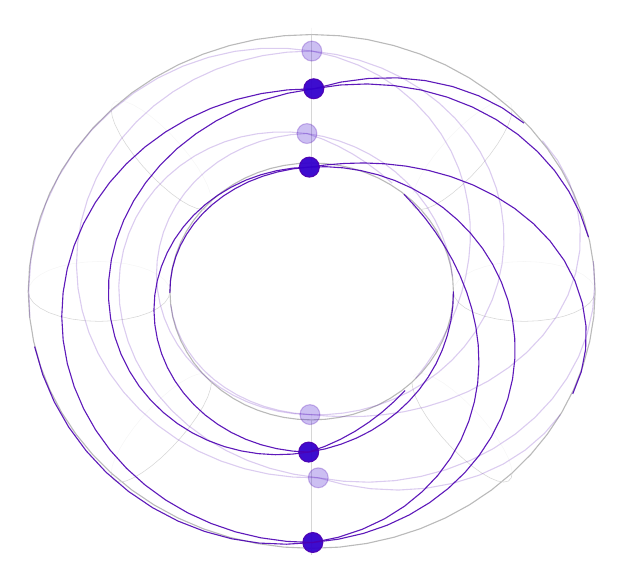
\begin{tikzpicture}[scale=0.9]
  \draw[gray!60, thin, opacity=0.9] (4.000,0.000) -- (3.981,0.355) -- (3.923,0.707) -- (3.828,1.052) -- (3.696,1.387) -- (3.528,1.709) -- (3.326,2.014) -- (3.092,2.300) -- (2.828,2.563) -- (2.538,2.802) -- (2.222,3.014) -- (1.886,3.197) -- (1.531,3.349) -- (1.161,3.469) -- (0.780,3.556) -- (0.392,3.608) -- (0.000,3.625) -- (-0.392,3.608) -- (-0.780,3.556) -- (-1.161,3.469) -- (-1.531,3.349) -- (-1.886,3.197) -- (-2.222,3.014) -- (-2.538,2.802) -- (-2.828,2.563) -- (-3.092,2.300) -- (-3.326,2.014) -- (-3.528,1.709) -- (-3.696,1.387) -- (-3.828,1.052) -- (-3.923,0.707) -- (-3.981,0.355) -- (-4.000,0.000) -- (-3.981,-0.355) -- (-3.923,-0.707) -- (-3.828,-1.052) -- (-3.696,-1.387) -- (-3.528,-1.709) -- (-3.326,-2.014) -- (-3.092,-2.300) -- (-2.828,-2.563) -- (-2.538,-2.802) -- (-2.222,-3.014) -- (-1.886,-3.197) -- (-1.531,-3.349) -- (-1.161,-3.469) -- (-0.780,-3.556) -- (-0.392,-3.608) -- (-0.000,-3.625) -- (0.392,-3.608) -- (0.780,-3.556) -- (1.161,-3.469) -- (1.531,-3.349) -- (1.886,-3.197) -- (2.222,-3.014) -- (2.538,-2.802) -- (2.828,-2.563) -- (3.092,-2.300) -- (3.326,-2.014) -- (3.528,-1.709) -- (3.696,-1.387) -- (3.828,-1.052) -- (3.923,-0.707) -- (3.981,-0.355) -- (4.000,-0.000);
  \draw[gray!60, thin, opacity=0.9] (2.000,-0.000) -- (1.990,0.178) -- (1.962,0.354) -- (1.914,0.526) -- (1.848,0.694) -- (1.764,0.854) -- (1.663,1.007) -- (1.546,1.150) -- (1.414,1.282) -- (1.269,1.401) -- (1.111,1.507) -- (0.943,1.599) -- (0.765,1.675) -- (0.581,1.735) -- (0.390,1.778) -- (0.196,1.804) -- (0.000,1.813) -- (-0.196,1.804) -- (-0.390,1.778) -- (-0.581,1.735) -- (-0.765,1.675) -- (-0.943,1.599) -- (-1.111,1.507) -- (-1.269,1.401) -- (-1.414,1.282) -- (-1.546,1.150) -- (-1.663,1.007) -- (-1.764,0.854) -- (-1.848,0.694) -- (-1.914,0.526) -- (-1.962,0.354) -- (-1.990,0.178) -- (-2.000,0.000) -- (-1.990,-0.178) -- (-1.962,-0.354) -- (-1.914,-0.526) -- (-1.848,-0.694) -- (-1.764,-0.854) -- (-1.663,-1.007) -- (-1.546,-1.150) -- (-1.414,-1.282) -- (-1.269,-1.401) -- (-1.111,-1.507) -- (-0.943,-1.599) -- (-0.765,-1.675) -- (-0.581,-1.735) -- (-0.390,-1.778) -- (-0.196,-1.804) -- (-0.000,-1.813) -- (0.196,-1.804) -- (0.390,-1.778) -- (0.581,-1.735) -- (0.765,-1.675) -- (0.943,-1.599) -- (1.111,-1.507) -- (1.269,-1.401) -- (1.414,-1.282) -- (1.546,-1.150) -- (1.663,-1.007) -- (1.764,-0.854) -- (1.848,-0.694) -- (1.914,-0.526) -- (1.962,-0.354) -- (1.990,-0.178) -- (2.000,-0.000);
  \draw[gray!35, very thin, opacity=0.9] (4.000,0.000) -- (3.981,-0.082) -- (3.924,-0.162) -- (3.831,-0.235) -- (3.707,-0.299) -- (3.556,-0.351) -- (3.383,-0.390) -- (3.195,-0.414) -- (3.000,-0.423) -- (2.805,-0.414) -- (2.617,-0.390) -- (2.444,-0.351) -- (2.293,-0.299) -- (2.169,-0.235) -- (2.076,-0.162) -- (2.019,-0.082) -- (2.000,-0.000);
  \draw[gray!35, very thin, opacity=0.2] (2.019,0.082) -- (2.076,0.162) -- (2.169,0.235) -- (2.293,0.299) -- (2.444,0.351) -- (2.617,0.390) -- (2.805,0.414) -- (3.000,0.423) -- (3.195,0.414) -- (3.383,0.390) -- (3.556,0.351) -- (3.707,0.299) -- (3.831,0.235) -- (3.924,0.162) -- (3.981,0.082) -- (4.000,0.000);
  \draw[gray!35, very thin, opacity=0.9] (2.828,2.563) -- (2.815,2.469) -- (2.775,2.353) -- (2.709,2.221) -- (2.621,2.077) -- (2.514,1.927) -- (2.392,1.777) -- (2.259,1.633) -- (2.121,1.500) -- (1.983,1.383) -- (1.851,1.287) -- (1.728,1.215) -- (1.621,1.171) -- (1.533,1.155) -- (1.468,1.169) -- (1.428,1.212) -- (1.414,1.282);
  \draw[gray!35, very thin, opacity=0.2] (1.428,1.376) -- (1.468,1.492) -- (1.533,1.625) -- (1.621,1.768) -- (1.728,1.918) -- (1.851,2.068) -- (1.983,2.212) -- (2.121,2.345) -- (2.259,2.462) -- (2.392,2.558) -- (2.514,2.630) -- (2.621,2.675) -- (2.709,2.690) -- (2.775,2.676) -- (2.815,2.634) -- (2.828,2.563);
  \draw[gray!35, very thin, opacity=0.9] (0.000,3.625) -- (0.000,3.525) -- (0.000,3.395) -- (0.000,3.238) -- (0.000,3.061) -- (0.000,2.871) -- (0.000,2.675) -- (0.000,2.481) -- (0.000,2.296) -- (0.000,2.128) -- (0.000,1.982) -- (0.000,1.864) -- (0.000,1.779) -- (0.000,1.731) -- (0.000,1.720) -- (0.000,1.748) -- (0.000,1.813);
  \draw[gray!35, very thin, opacity=0.2] (0.000,1.912) -- (0.000,2.043) -- (0.000,2.200) -- (0.000,2.377) -- (0.000,2.567) -- (0.000,2.763) -- (0.000,2.957) -- (0.000,3.142) -- (0.000,3.310) -- (0.000,3.456) -- (0.000,3.574) -- (0.000,3.659) -- (0.000,3.707) -- (0.000,3.718) -- (0.000,3.690) -- (0.000,3.625);
  \draw[gray!35, very thin, opacity=0.9] (-2.828,2.563) -- (-2.815,2.469) -- (-2.775,2.353) -- (-2.709,2.221) -- (-2.621,2.077) -- (-2.514,1.927) -- (-2.392,1.777) -- (-2.259,1.633) -- (-2.121,1.500) -- (-1.983,1.383) -- (-1.851,1.287) -- (-1.728,1.215) -- (-1.621,1.171) -- (-1.533,1.155) -- (-1.468,1.169) -- (-1.428,1.212) -- (-1.414,1.282);
  \draw[gray!35, very thin, opacity=0.2] (-1.428,1.376) -- (-1.468,1.492) -- (-1.533,1.625) -- (-1.621,1.768) -- (-1.728,1.918) -- (-1.851,2.068) -- (-1.983,2.212) -- (-2.121,2.345) -- (-2.259,2.462) -- (-2.392,2.558) -- (-2.514,2.630) -- (-2.621,2.675) -- (-2.709,2.690) -- (-2.775,2.676) -- (-2.815,2.634) -- (-2.828,2.563);
  \draw[gray!35, very thin, opacity=0.9] (-4.000,0.000) -- (-3.981,-0.082) -- (-3.924,-0.162) -- (-3.831,-0.235) -- (-3.707,-0.299) -- (-3.556,-0.351) -- (-3.383,-0.390) -- (-3.195,-0.414) -- (-3.000,-0.423) -- (-2.805,-0.414) -- (-2.617,-0.390) -- (-2.444,-0.351) -- (-2.293,-0.299) -- (-2.169,-0.235) -- (-2.076,-0.162) -- (-2.019,-0.082) -- (-2.000,0.000);
  \draw[gray!35, very thin, opacity=0.2] (-2.019,0.082) -- (-2.076,0.162) -- (-2.169,0.235) -- (-2.293,0.299) -- (-2.444,0.351) -- (-2.617,0.390) -- (-2.805,0.414) -- (-3.000,0.423) -- (-3.195,0.414) -- (-3.383,0.390) -- (-3.556,0.351) -- (-3.707,0.299) -- (-3.831,0.235) -- (-3.924,0.162) -- (-3.981,0.082) -- (-4.000,0.000);
  \draw[gray!35, very thin, opacity=0.9] (-2.828,-2.563) -- (-2.815,-2.634) -- (-2.775,-2.676) -- (-2.709,-2.690) -- (-2.621,-2.675) -- (-2.514,-2.630) -- (-2.392,-2.558) -- (-2.259,-2.462) -- (-2.121,-2.345) -- (-1.983,-2.212) -- (-1.851,-2.068) -- (-1.728,-1.918) -- (-1.621,-1.768) -- (-1.533,-1.625) -- (-1.468,-1.492) -- (-1.428,-1.376) -- (-1.414,-1.282);
  \draw[gray!35, very thin, opacity=0.2] (-1.428,-1.212) -- (-1.468,-1.169) -- (-1.533,-1.155) -- (-1.621,-1.171) -- (-1.728,-1.215) -- (-1.851,-1.287) -- (-1.983,-1.383) -- (-2.121,-1.500) -- (-2.259,-1.633) -- (-2.392,-1.777) -- (-2.514,-1.927) -- (-2.621,-2.077) -- (-2.709,-2.221) -- (-2.775,-2.353) -- (-2.815,-2.469) -- (-2.828,-2.563);
  \draw[gray!35, very thin, opacity=0.9] (-0.000,-3.625) -- (-0.000,-3.690) -- (-0.000,-3.718) -- (-0.000,-3.707) -- (-0.000,-3.659) -- (-0.000,-3.574) -- (-0.000,-3.456) -- (-0.000,-3.310) -- (-0.000,-3.142) -- (-0.000,-2.957) -- (-0.000,-2.763) -- (-0.000,-2.567) -- (-0.000,-2.377) -- (-0.000,-2.200) -- (-0.000,-2.043) -- (-0.000,-1.912) -- (-0.000,-1.813);
  \draw[gray!35, very thin, opacity=0.2] (-0.000,-1.748) -- (-0.000,-1.720) -- (-0.000,-1.731) -- (-0.000,-1.779) -- (-0.000,-1.864) -- (-0.000,-1.982) -- (-0.000,-2.128) -- (-0.000,-2.296) -- (-0.000,-2.481) -- (-0.000,-2.675) -- (-0.000,-2.871) -- (-0.000,-3.061) -- (-0.000,-3.238) -- (-0.000,-3.395) -- (-0.000,-3.525) -- (-0.000,-3.625);
  \draw[gray!35, very thin, opacity=0.9] (2.828,-2.563) -- (2.815,-2.634) -- (2.775,-2.676) -- (2.709,-2.690) -- (2.621,-2.675) -- (2.514,-2.630) -- (2.392,-2.558) -- (2.259,-2.462) -- (2.121,-2.345) -- (1.983,-2.212) -- (1.851,-2.068) -- (1.728,-1.918) -- (1.621,-1.768) -- (1.533,-1.625) -- (1.468,-1.492) -- (1.428,-1.376) -- (1.414,-1.282);
  \draw[gray!35, very thin, opacity=0.2] (1.428,-1.212) -- (1.468,-1.169) -- (1.533,-1.155) -- (1.621,-1.171) -- (1.728,-1.215) -- (1.851,-1.287) -- (1.983,-1.383) -- (2.121,-1.500) -- (2.259,-1.633) -- (2.392,-1.777) -- (2.514,-1.927) -- (2.621,-2.077) -- (2.709,-2.221) -- (2.775,-2.353) -- (2.815,-2.469) -- (2.828,-2.563);
  \filldraw[fill=violet!40!blue, draw=violet!60!blue, opacity=0.25] (0.093,-2.630) circle (4pt); % v8
  \filldraw[fill=violet!40!blue, draw=violet!60!blue, opacity=0.25] (-0.025,-1.738) circle (4pt); % v7
  \draw[violet!60!blue, opacity=0.2] (-0.067,2.228) -- (-0.298,2.249) -- (-0.532,2.248) -- (-0.767,2.225) -- (-0.999,2.180) -- (-1.226,2.112) -- (-1.447,2.021) -- (-1.657,1.909) -- (-1.856,1.774) -- (-2.040,1.619) -- (-2.207,1.445) -- (-2.354,1.252) -- (-2.480,1.042) -- (-2.581,0.817) -- (-2.656,0.580) -- (-2.703,0.332) -- (-2.722,0.077) -- (-2.709,-0.184) -- (-2.666,-0.447) -- (-2.590,-0.708) -- (-2.483,-0.966) -- (-2.343,-1.216) -- (-2.173,-1.455) -- (-1.973,-1.681) -- (-1.744,-1.890) -- (-1.488,-2.078) -- (-1.209,-2.244) -- (-0.908,-2.384) -- (-0.588,-2.497) -- (-0.253,-2.579) -- (0.093,-2.630);
  \draw[violet!60!blue, opacity=0.2] (0.002,3.392) -- (-0.346,3.376) -- (-0.690,3.328) -- (-1.027,3.246) -- (-1.353,3.133) -- (-1.664,2.990) -- (-1.957,2.817) -- (-2.228,2.618) -- (-2.474,2.393) -- (-2.693,2.146) -- (-2.883,1.879) -- (-3.040,1.596) -- (-3.163,1.299) -- (-3.252,0.991) -- (-3.304,0.677) -- (-3.319,0.360) -- (-3.297,0.042) -- (-3.238,-0.271) -- (-3.144,-0.578) -- (-3.014,-0.874) -- (-2.850,-1.156) -- (-2.654,-1.420) -- (-2.429,-1.665) -- (-2.176,-1.887) -- (-1.899,-2.084) -- (-1.600,-2.253) -- (-1.283,-2.392) -- (-0.951,-2.501) -- (-0.609,-2.577) -- (-0.260,-2.620) -- (0.093,-2.630);
  \draw[violet!60!blue, opacity=0.2] (-0.025,-1.738) -- (0.208,-1.738) -- (0.444,-1.717) -- (0.680,-1.675) -- (0.915,-1.611) -- (1.146,-1.525) -- (1.371,-1.418) -- (1.587,-1.289) -- (1.791,-1.139) -- (1.980,-0.970) -- (2.153,-0.781) -- (2.307,-0.575) -- (2.439,-0.354) -- (2.548,-0.118) -- (2.631,0.130) -- (2.686,0.387) -- (2.712,0.651) -- (2.708,0.919) -- (2.673,1.189) -- (2.606,1.456) -- (2.507,1.719) -- (2.376,1.974) -- (2.214,2.217) -- (2.022,2.445) -- (1.801,2.656) -- (1.554,2.846) -- (1.281,3.012) -- (0.987,3.152) -- (0.673,3.263) -- (0.344,3.344) -- (0.002,3.392);
  \filldraw[fill=violet!40!blue, draw=violet!60!blue, opacity=0.95] (0.016,-3.543) circle (4pt); % v5
  \draw[violet!60!blue, opacity=0.2] (-0.067,2.228) -- (-0.292,2.212) -- (-0.514,2.174) -- (-0.731,2.116) -- (-0.940,2.038) -- (-1.139,1.941) -- (-1.326,1.826) -- (-1.498,1.693) -- (-1.655,1.546) -- (-1.794,1.384) -- (-1.914,1.211) -- (-2.014,1.027) -- (-2.092,0.835) -- (-2.147,0.636) -- (-2.180,0.433) -- (-2.190,0.229) -- (-2.176,0.024) -- (-2.139,-0.178) -- (-2.080,-0.376) -- (-1.998,-0.567) -- (-1.894,-0.749) -- (-1.771,-0.921) -- (-1.628,-1.080) -- (-1.469,-1.225) -- (-1.293,-1.355) -- (-1.104,-1.467) -- (-0.903,-1.561) -- (-0.692,-1.636) -- (-0.474,-1.691) -- (-0.250,-1.725) -- (-0.025,-1.738);
  \filldraw[fill=violet!40!blue, draw=violet!60!blue, opacity=0.95] (-0.042,-2.267) circle (4pt); % v6
  \draw[violet!60!blue, opacity=0.9] (-0.042,-2.267) -- (0.187,-2.186) -- (0.404,-2.088) -- (0.610,-1.975) -- (0.804,-1.848) -- (0.987,-1.709) -- (1.158,-1.558) -- (1.318,-1.398);
  \draw[violet!60!blue, opacity=0.2] (1.467,-1.227) -- (1.606,-1.047) -- (1.733,-0.858) -- (1.849,-0.660) -- (1.952,-0.453) -- (2.042,-0.237) -- (2.117,-0.012) -- (2.176,0.220) -- (2.217,0.461) -- (2.238,0.708) -- (2.236,0.960) -- (2.210,1.216) -- (2.158,1.473) -- (2.077,1.729) -- (1.967,1.980) -- (1.825,2.224) -- (1.653,2.457) -- (1.449,2.674) -- (1.214,2.872) -- (0.949,3.047) -- (0.657,3.194) -- (0.340,3.310) -- (0.002,3.392);
  \draw[violet!60!blue, opacity=0.2] (-0.025,-1.738) -- (0.212,-1.758) -- (0.463,-1.767) -- (0.730,-1.763) -- (1.010,-1.740) -- (1.301,-1.698) -- (1.600,-1.631) -- (1.903,-1.537) -- (2.204,-1.414) -- (2.497,-1.261) -- (2.777,-1.076) -- (3.035,-0.861) -- (3.266,-0.616) -- (3.461,-0.346) -- (3.616,-0.053) -- (3.725,0.258) -- (3.784,0.580) -- (3.788,0.907) -- (3.737,1.233) -- (3.631,1.550) -- (3.469,1.850) -- (3.256,2.127);
  \draw[violet!60!blue, opacity=0.9] (2.996,2.375) -- (2.693,2.588) -- (2.355,2.761) -- (1.989,2.891) -- (1.603,2.975) -- (1.206,3.014) -- (0.806,3.006) -- (0.412,2.954) -- (0.030,2.860);
  \draw[violet!60!blue, opacity=0.2] (0.002,3.392) -- (-0.351,3.430) -- (-0.714,3.429) -- (-1.083,3.388) -- (-1.453,3.304) -- (-1.817,3.179) -- (-2.171,3.011) -- (-2.507,2.803) -- (-2.821,2.556) -- (-3.107,2.273) -- (-3.360,1.957) -- (-3.576,1.612) -- (-3.750,1.242) -- (-3.879,0.854) -- (-3.961,0.452) -- (-3.993,0.042) -- (-3.976,-0.370);
  \draw[violet!60!blue, opacity=0.9] (-3.910,-0.778) -- (-3.795,-1.175) -- (-3.633,-1.557) -- (-3.427,-1.917) -- (-3.181,-2.251) -- (-2.899,-2.554) -- (-2.585,-2.822) -- (-2.245,-3.052) -- (-1.885,-3.241) -- (-1.510,-3.387) -- (-1.127,-3.491) -- (-0.741,-3.551) -- (-0.358,-3.567) -- (0.016,-3.543);
  \draw[violet!60!blue, opacity=0.2] (0.093,-2.630) -- (0.447,-2.678) -- (0.809,-2.692) -- (1.175,-2.670) -- (1.540,-2.611) -- (1.897,-2.515) -- (2.243,-2.383) -- (2.570,-2.214) -- (2.875,-2.012) -- (3.151,-1.778) -- (3.395,-1.516) -- (3.601,-1.228) -- (3.767,-0.920) -- (3.889,-0.595) -- (3.965,-0.259) -- (3.993,0.084) -- (3.974,0.427);
  \draw[violet!60!blue, opacity=0.9] (3.906,0.766) -- (3.791,1.095) -- (3.631,1.409) -- (3.429,1.703) -- (3.187,1.973) -- (2.910,2.215) -- (2.602,2.426) -- (2.268,2.602) -- (1.914,2.741) -- (1.545,2.842) -- (1.166,2.904) -- (0.783,2.928) -- (0.403,2.913) -- (0.030,2.860);
  \draw[violet!60!blue, opacity=0.9] (-0.042,-2.267) -- (0.191,-2.222) -- (0.417,-2.155) -- (0.633,-2.069) -- (0.838,-1.965) -- (1.030,-1.842) -- (1.208,-1.704) -- (1.371,-1.551) -- (1.517,-1.386) -- (1.644,-1.209) -- (1.754,-1.022) -- (1.843,-0.827) -- (1.913,-0.625) -- (1.963,-0.419) -- (1.992,-0.209) -- (2.000,0.001);
  \draw[violet!60!blue, opacity=0.2] (1.988,0.212) -- (1.954,0.421) -- (1.901,0.626) -- (1.827,0.825) -- (1.734,1.018) -- (1.622,1.202) -- (1.491,1.377) -- (1.343,1.539) -- (1.180,1.688) -- (1.001,1.823) -- (0.808,1.941) -- (0.603,2.042) -- (0.388,2.124) -- (0.164,2.187) -- (-0.067,2.228);
  \draw[violet!60!blue, opacity=0.9] (-0.033,1.754) -- (-0.262,1.730) -- (-0.482,1.686) -- (-0.692,1.625) -- (-0.891,1.547) -- (-1.076,1.453) -- (-1.247,1.346) -- (-1.403,1.225) -- (-1.542,1.094) -- (-1.664,0.953) -- (-1.767,0.803) -- (-1.853,0.647) -- (-1.919,0.485) -- (-1.966,0.319) -- (-1.993,0.150) -- (-2.001,-0.019);
  \draw[violet!60!blue, opacity=0.2] (-1.989,-0.188) -- (-1.958,-0.355) -- (-1.907,-0.519) -- (-1.837,-0.679) -- (-1.749,-0.832) -- (-1.643,-0.978) -- (-1.520,-1.115) -- (-1.380,-1.242) -- (-1.224,-1.357) -- (-1.053,-1.460) -- (-0.869,-1.548) -- (-0.673,-1.622) -- (-0.465,-1.678) -- (-0.249,-1.717) -- (-0.025,-1.738);
  \draw[violet!60!blue, opacity=0.2] (0.093,-2.630) -- (0.455,-2.725) -- (0.833,-2.784) -- (1.221,-2.803) -- (1.611,-2.778) -- (1.993,-2.708) -- (2.360,-2.594) -- (2.703,-2.436) -- (3.014,-2.238) -- (3.285,-2.003) -- (3.510,-1.737);
  \draw[violet!60!blue, opacity=0.9] (3.684,-1.445) -- (3.804,-1.135) -- (3.866,-0.814) -- (3.871,-0.489) -- (3.820,-0.167) -- (3.716,0.144) -- (3.563,0.438) -- (3.365,0.710) -- (3.131,0.955) -- (2.865,1.170) -- (2.577,1.353) -- (2.272,1.504) -- (1.959,1.622) -- (1.644,1.709) -- (1.332,1.768) -- (1.030,1.801) -- (0.740,1.813) -- (0.465,1.806) -- (0.207,1.786) -- (-0.033,1.754);
  \draw[violet!60!blue, opacity=0.9] (0.016,-3.543) -- (0.376,-3.469) -- (0.715,-3.356) -- (1.028,-3.209) -- (1.311,-3.030) -- (1.562,-2.824) -- (1.779,-2.597) -- (1.960,-2.352) -- (2.107,-2.095) -- (2.218,-1.829) -- (2.296,-1.558) -- (2.343,-1.287) -- (2.360,-1.018) -- (2.350,-0.754) -- (2.316,-0.497) -- (2.261,-0.249) -- (2.187,-0.010) -- (2.096,0.218) -- (1.991,0.436) -- (1.873,0.644) -- (1.744,0.840) -- (1.606,1.027) -- (1.458,1.204) -- (1.302,1.371);
  \draw[violet!60!blue, opacity=0.2] (1.136,1.528) -- (0.961,1.675) -- (0.776,1.812) -- (0.582,1.937) -- (0.376,2.049) -- (0.160,2.147) -- (-0.067,2.228);
  \filldraw[fill=violet!40!blue, draw=violet!60!blue, opacity=0.25] (-0.067,2.228) circle (4pt); % v3
  \filldraw[fill=violet!40!blue, draw=violet!60!blue, opacity=0.25] (0.002,3.392) circle (4pt); % v4
  \draw[violet!60!blue, opacity=0.9] (-0.033,1.754) -- (-0.265,1.740) -- (-0.493,1.704) -- (-0.715,1.647) -- (-0.930,1.570) -- (-1.135,1.472) -- (-1.327,1.356) -- (-1.505,1.223) -- (-1.667,1.074) -- (-1.811,0.910) -- (-1.935,0.735) -- (-2.038,0.548) -- (-2.120,0.353) -- (-2.179,0.151) -- (-2.214,-0.055) -- (-2.226,-0.263) -- (-2.213,-0.471) -- (-2.177,-0.677) -- (-2.118,-0.878) -- (-2.036,-1.073) -- (-1.932,-1.259) -- (-1.808,-1.433) -- (-1.664,-1.596) -- (-1.503,-1.744) -- (-1.326,-1.875) -- (-1.134,-1.990) -- (-0.931,-2.086) -- (-0.718,-2.162) -- (-0.497,-2.218) -- (-0.271,-2.253) -- (-0.042,-2.267);
  \draw[violet!60!blue, opacity=0.9] (0.016,-3.543) -- (0.379,-3.496) -- (0.729,-3.415) -- (1.063,-3.300) -- (1.376,-3.154) -- (1.665,-2.980) -- (1.927,-2.780) -- (2.160,-2.558) -- (2.362,-2.317) -- (2.531,-2.060) -- (2.667,-1.792) -- (2.768,-1.515) -- (2.835,-1.233) -- (2.867,-0.949) -- (2.866,-0.668) -- (2.833,-0.392) -- (2.769,-0.124) -- (2.676,0.134) -- (2.556,0.378) -- (2.412,0.606) -- (2.245,0.817) -- (2.059,1.009) -- (1.857,1.180) -- (1.640,1.330) -- (1.412,1.458) -- (1.176,1.564) -- (0.935,1.646) -- (0.691,1.706) -- (0.446,1.744) -- (0.204,1.760) -- (-0.033,1.754);
  \draw[violet!60!blue, opacity=0.9] (0.030,2.860) -- (-0.342,2.844) -- (-0.710,2.792) -- (-1.071,2.706) -- (-1.419,2.585) -- (-1.751,2.433) -- (-2.063,2.250) -- (-2.353,2.038) -- (-2.616,1.800) -- (-2.850,1.538) -- (-3.053,1.255) -- (-3.221,0.955) -- (-3.354,0.641) -- (-3.450,0.316) -- (-3.508,-0.017) -- (-3.527,-0.353) -- (-3.507,-0.688) -- (-3.448,-1.020) -- (-3.351,-1.345) -- (-3.217,-1.658) -- (-3.048,-1.956) -- (-2.846,-2.237) -- (-2.612,-2.497) -- (-2.349,-2.733) -- (-2.061,-2.943) -- (-1.750,-3.124) -- (-1.420,-3.274) -- (-1.074,-3.393) -- (-0.717,-3.477) -- (-0.353,-3.527) -- (0.016,-3.543);
  \draw[violet!60!blue, opacity=0.9] (0.030,2.860) -- (-0.336,2.797) -- (-0.689,2.699) -- (-1.025,2.570) -- (-1.341,2.411) -- (-1.633,2.225) -- (-1.899,2.016) -- (-2.135,1.785) -- (-2.340,1.538) -- (-2.513,1.277) -- (-2.652,1.005) -- (-2.757,0.727) -- (-2.827,0.446) -- (-2.863,0.165) -- (-2.866,-0.112) -- (-2.837,-0.382) -- (-2.777,-0.642) -- (-2.689,-0.889) -- (-2.573,-1.122) -- (-2.434,-1.338) -- (-2.272,-1.534) -- (-2.091,-1.710) -- (-1.894,-1.865) -- (-1.683,-1.997) -- (-1.460,-2.105) -- (-1.230,-2.190) -- (-0.993,-2.251) -- (-0.754,-2.289) -- (-0.514,-2.304) -- (-0.276,-2.296) -- (-0.042,-2.267);
  \filldraw[fill=violet!40!blue, draw=violet!60!blue, opacity=0.95] (-0.033,1.754) circle (4pt); % v2
  \filldraw[fill=violet!40!blue, draw=violet!60!blue, opacity=0.95] (0.030,2.860) circle (4pt); % v1
\end{tikzpicture}
            \end{center}
\caption{A drawing of $K_{4,4}$ on a torus (3D-version)}\label{K44:3d}
        \end{figure}

To understand why we can't draw $K_{5,5}$ on the torus without edge crossings we can use a similar Euler characteristic argument as we gave for $K_8$. 

Suppose we could draw $K_{5,5}$ on the torus without edge crossings. Then $V = 5 + 5 = 10$ and $E = 5 \times 5 = 25$. Any face containing exactly 3 edges is a triangle, but $K_{5,5}$ does not contain any triangles (this is true of all utility graphs). So every face in a drawing of $K_{5,5}$ must contain at least 4 edges. Hence we have
the new inequality $F \le 2E/4 = E/2$. So in the case of $K_{5,5}$, $F \le 25/2$. But then
\[
V- E + F \le 10 - 25 + \frac{25}{2} = -5/2 <0,
\] contradicting the Euler characteristic bound (\ref{EC:eq}).
\fi

\end{document}

